The tidal forces induced by a planet embedded in a gas disk result in the excitation of sound waves \citep{goldreich1980}.
These waves propagate freely through the disk, interfering with one another and eventually steepening into shock waves \citep{goodman2001}.
The overall result is the formation of a coherent, one-armed spiral density wave connected to the planet, known as the \textit{planet wake} \citep{ogilvie2002}. 
This chapter provides an outline of the theory behind this interaction, and introduces the method with which we will go on to construct semi-analytic models of the planet wake.
These ideas also provide the necessary foundation that will allow us to go on to detecting and measuring young planets through kinematic observations.

\section{Spiral Density Waves}

\begin{figure}
    \centering
    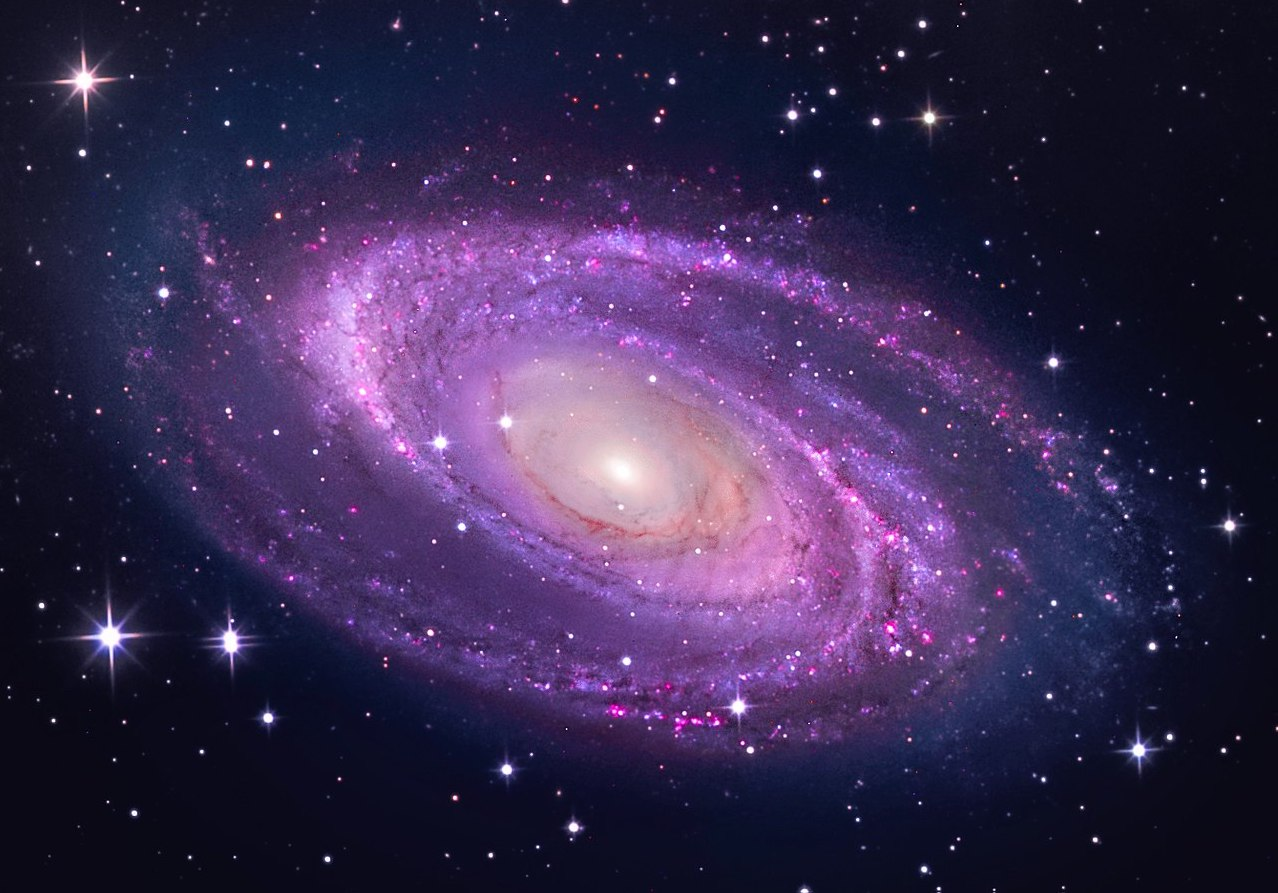
\includegraphics[width = 0.7\textwidth]{figures/M81.jpeg}
    \caption{Long exposure image of Messier 81 taken through a 20 inch telescope by astrophotographer \citet{adler2015}, taken with LRGB filters and a Hydrogen-$\alpha$ filter that was assigned to red. Overall 20 hours of exposures were taken.}
    \label{fig:M81}
\end{figure}

Perhaps the most well known examples of spiral structures in astrophysics are the grand design spirals of galaxies like Messier 81 (M81), shown in Figure \ref{fig:M81}.
The disk of a galaxy rotates differentially, similarly to a circumstellar disk, resulting in an initially puzzling state of affairs.
If the material making up the spiral structure remains in the arm, then the pattern should be quickly destroyed since material in the inner disk orbits at a much greater rate than that in the outer disk.
This is known at the \textit{winding problem}, and it proved to be a serious challenge for early attempts to explain spiral structure in galaxies \citep{wilczynski1896,oort1962}.

The first major advance in our understanding of the origins of galactic spiral structure was made by Bertil Lindblad in the early 1960s. 
Lindblad proposed that spiral structure may be a quasi-stationary wave resulting from the superposition of multiple spiral modes.
In Lindblad's model, these modes were excited through the interaction of orbital motions and gravitational forces of the stars in the disk \citep{lindblad1963}.
This was a radical view at the time, as it was widely believed that spiral structure was induced by galactic-scale magnetic fields \citep[eg.][]{hoyle1961,oki1964}.
The paradigm-shift would come shortly after with the seminal work by \citet{lin1964}, pioneering the \textit{density wave theory} picture of spiral structure.
In their view, spiral arms are quasi-static overdense regions of the disk resulting from periodic compression and rarefaction of disk material, similar to a traffic jam.
This, in combination with Lindblad's findings make up the \textit{Lin-Shu Hypothesis}, which states that galactic spiral structure is a stationary density wave, and that the spiral pattern is unchanged over long timescales apart from the overall rotation of the galaxy.
A more precise statement of the hypothesis is that the spiral is a marginally stable wave mode of the disk.

The Lin-Shu hypothesis is however not correct.
The spiral structure found in galaxies is indeed a density wave, but the wave is not a stationary, stable mode of the disk.
Instead the spiral arms are the result of the disk responding to a variety of gravitational disturbances such as nearby galaxies \citep{goldreich1965,julian1966}.
Indeed, the grand design spirals in M81 are thought to be the result of tidal-interactions with its companion galaxy Messier 82 \citep{yun1999a}.

Spiral arms similar to those found in galaxies have been observed in the disks around the stars HD 142529 \citep{christiaens2014}, MWC 758 \citep{benisty2015}, Elias 27 \citep{perez2016,huang2018}, IM Lupi \citep{avenhaus2018,huang2018}, WaOph 6 \citep{huang2018}, HD 163296 \citep{calcino2022}, TW Hya \citep{teague2022} and others \citep[and references therin]{dong2018}.
Figure \ref{fig:mwc758} shows the double-armed spiral of MWC 758 in scattered light.
The origin of most of these spirals is still unknown \citep[eg.][]{zhang2018}.
Of particular interest to us here are kinematic detections of planets located inside dust gaps \citep{pinte2018a,pinte2019,pinte2020,teague2021,teague2022}, since they are very well explained by the planet wake scenario, as we will see.

\begin{figure}
    \centering
    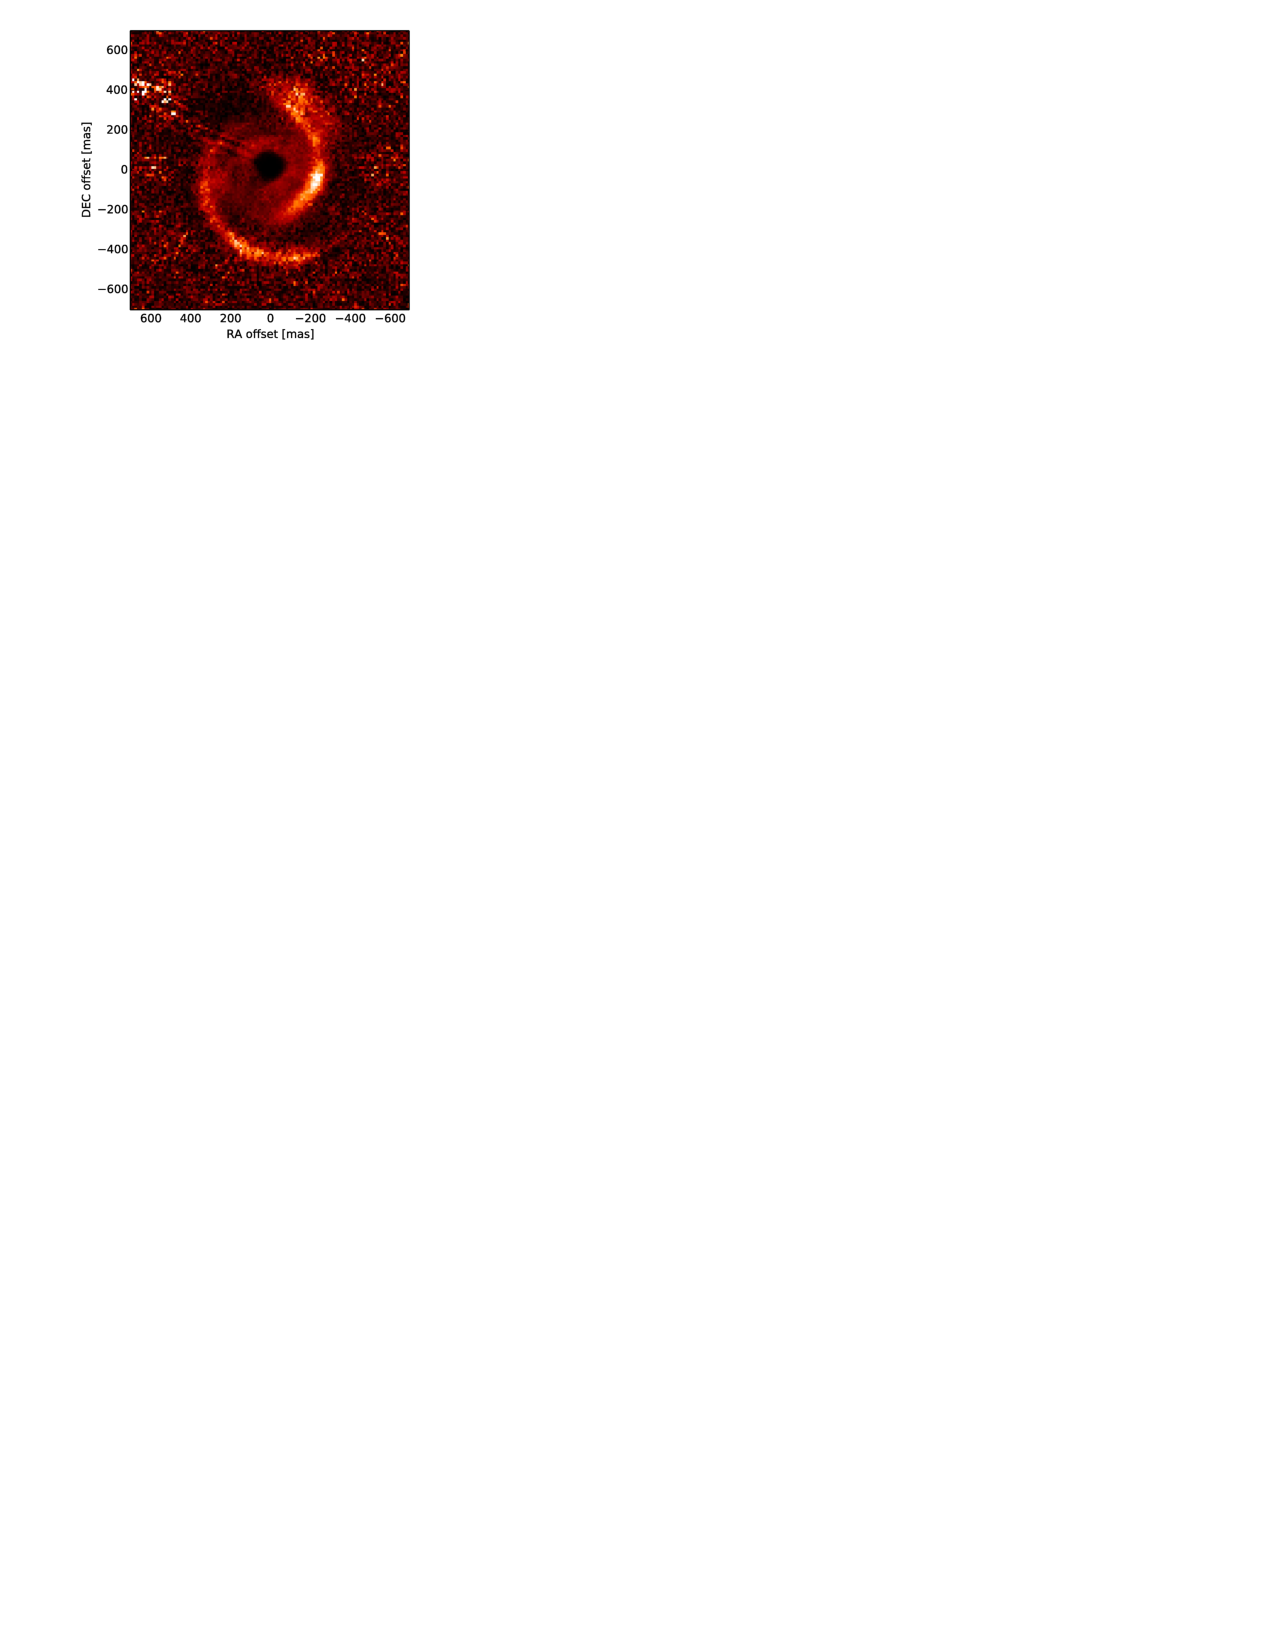
\includegraphics[width = 0.7\textwidth]{figures/mwc758.pdf}
    \caption{Polarised intensity image of the disk MWC 758 obtained in December 2014 with SPHERE \citep[eg.][]{beuzit2019}. The colour scale is arbitrary. Two large spiral arms are clearly present in the disk \citep{benisty2015}. The origin of these spiral arms is still unknown.}
    \label{fig:mwc758}
\end{figure}

\subsection{Spiral Structure Preliminaries}
We now introduce the following concepts:
\begin{enumerate}
    \item The \textit{pitch angle} $\alpha$: of a spiral arm is defined as the angle between the tangent to the spiral at some radius $r$ and the circle with the same radius. 
    Thus $\alpha$ is in general a function of radius and $0 < \alpha < \pi/2$ by definition.
    \item $m$-fold \textit{rotational symmetry}: if a rotation of $2\pi/m$ radians results in no change to the disk surface density, that is $\Sigma(r,\phi)=\Sigma(r,\phi+\frac{2\pi}{m})$, then the disk is said to contain $m$ spiral arms and exhibits an $m$-fold rotational symmetry. 
    For example, a disk containing two spiral arms will be unchanged under a rotation of $180^\circ$ and so has $2$-fold rotational symmetry.
    \item \textit{Leading} and \textit{trailing} spiral arms: the tip of a leading spiral arm points in the direction of the bulk rotation of the disk, while the tip of a trailing arm points in the opposite direction to the rotation. 
    While it seems that leading arms may indeed be physically realised in the universe \citep[eg.][]{vaisanen2008}, they are at minimum very rare. 
    We will be concerned only with trailing spirals in this thesis.
%    \item The \textit{pattern speed} $\Omega_\mathrm{p}$: In the Lin-Shu hypothesis the spiral structure is a fixed pattern that rotates rigidly. 
%    The angular speed of rotation of these spirals according to some inertial observer is known as the pattern speed $\Omega_\mathrm{p}$. 
%    More generally, the pattern speed is well defined so long as the spirals constitute a steady state solution in some rigidly rotating frame. 
%    As we will see, this is the case for the spiral wake generated by a perturbing planet on a circular orbit, in which case the pattern speed is simply equal to the orbital rotation of the planet
\end{enumerate}

Consider a disk containing a set of $m$ spiral arms such that is has $m$-fold symmetry. We may parameterise the curves defined by the centre of each of the spiral arms as
\begin{align}
    m\phi + f(r,t) = C \,\, \mathrm{mod} \,\, 2\pi, \label{eq:spiral_para}
\end{align}
where $C$ is a constant real number and $f$ is known as the \textit{shape function}. The \textit{radial wavenumber} $k$ is defined in terms of $f$ and is given by
\begin{align}
    k(r,t) \equiv \partial_r f(r,t).
\end{align}
For a counter-clockwise rotating disk we have $m>0$ and so $k>0$ corresponds to trailing arms while $k<0$ gives leading arms. 
The opposite is true for clockwise rotating disks with $m<0$. 
We will always assume both $k$ and $m$ are positive, corresponding to tailing arms in a counter-clockwise rotating disk. 
The pitch angle $\alpha$ of a spiral arm is given by
\begin{align}
    \mathrm{cot}\,\alpha = \left| r \partial_r \phi \right|,
\end{align}
where $r \partial_r \phi$ is evaluated along the curve that defines the spiral. In terms of the parameterisation \ref{eq:spiral_para} we have $\partial_r[m\phi+f(r,t)] = m \partial_r \phi + k = 0$ giving
\begin{align}
    \alpha = \arctan \left( \frac{m}{kr} \right). \label{eq:pitchangle}
\end{align}

\subsection{No Leading Spirals}

In the previous section we stated that while leading spirals may exist in nature, they are at least much rarer that than trailing spirals. 
Indeed, there are \textbf{no} known examples of leading spirals in circumstellar disks.
This is at least initially surprising; if the trailing spiral arms seen in astrophysical disks are steady-state solutions governed by Newtonian physics, which is fully time-reversible, surely the corresponding leading spirals solution is entirely equivalent?
\citet{lynden-bell1967} followed this argument to prove the \textit{anti-spiral} theorem, which states that if trailing spirals constitute a steady-state solution to time-reversible equations, then there necessarily exists an equivalent leading spiral solution.
Thus the apparent ubiquity of trailing spirals in nature tells us that either the governing physics is not time-reversible, or the spirals are not true steady-state solutions.
In the latter case spiral structure may be the result of a recent disturbance, or may be continuously regenerated for example by period tidal forcing.
This mimics the failing of the Lin-Shu hypothesis for galaxies, where spiral structure turned out to be the response of the disk to disturbances.
In the section \ref{sec:planet_forcing} we will see that the perturbations driven periodically by a gravitating body embedded in a circumstellar disk result in a trailing spiral structure.

\section{The Linear Disk Response}

Before determining how the periodic forcing of the planet potential perturbs the disk, we must first determine how the disk responds to some small, generic disturbance.
The 2D inviscid equations of momentum and continuity expressed in terms of surface density are given by \citep{landau1959}
\begin{align}
    &\partial_t u + u \partial_r u + \frac{v}{r} \partial_\phi u - \frac{v^2}{r} = - \partial_r \Phi - \frac{1}{\Sigma} \partial_r P, \label{eq:mom_eq_u} \\ 
    &\partial_t v + u \partial_r v + \frac{v}{r} \partial_\phi v - \frac{uv}{r} = - \frac{1}{r} \partial_\phi \Phi - \frac{1}{r\Sigma} \partial_\phi P, \label{eq:mom_eq_v} \\
    &\partial_t \Sigma + \frac{1}{r} \partial_r (r \Sigma u) + \frac{1}{r} \partial_\phi (\Sigma v) = 0. 
    \label{eq:cont_2d}
\end{align}
Assuming a polytropic equation of state
\begin{align}
    P = K \Sigma^\gamma,
\end{align}
where $K$ is a constant and $\gamma$ is the adiabatic index. We then find the sound speed $c$ to be
\begin{align}
    c^2 = \partial_\Sigma P = \gamma K \Sigma^{\gamma-1}. \label{eq:cs_poly}
\end{align}
To simplify the equations we introduce the specific enthalpy $h$. Since the equation of state we are using is isentropic, we have $dh = dP / \Sigma$ giving
\begin{align}
    h = \int \frac{1}{\Sigma} dP = \int \frac{c^2}{\Sigma} d\Sigma = \frac{\gamma}{\gamma-1} K \Sigma^{\gamma-1}. \label{eq:enthalpy}
\end{align}
Note that
\begin{align}
    \partial_x h = \frac{\gamma}{\gamma - 1} K \partial_\Sigma (\Sigma^{\gamma-1}) \partial_x \Sigma = \gamma K \Sigma^{\gamma-2} \partial_x \Sigma,
\end{align}
such that the right-hand sides of equations \ref{eq:mom_eq_u} and \ref{eq:mom_eq_v} become
\begin{align}
    - \partial_r \Phi - \frac{1}{\Sigma} \partial_r P = - \partial_r \Phi - \gamma K \Sigma^{\gamma-2} \partial_r \Sigma = - \partial_r (\Phi + h) \label{eq:mom_u_RHS},
\end{align}
and
\begin{align}
    - \frac{1}{r} \partial_\phi \Phi - \frac{1}{r\Sigma} \partial_\phi P = - \frac{1}{r} \partial_\phi (\Phi + h) \label{eq:mom_v_RHS},
\end{align}
respectively.

We now perform a linear perturbation study; we assume that the spiral waves in the disk constitute only a small perturbation from some background steady-state, and that the background state is axisymmetric.
We rewrite the quantities $\Sigma,\Phi,h,u,v$ as a combination of the background value (denoted by subscript 0) and a small perturbation  (denoted by $\delta$)
\begin{align}
    \Sigma &= \Sigma_0 + \delta\Sigma, \label{eq:pertsig} \\
    \Phi &= \Phi_0 + \delta\Phi, \label{eq:pertphi} \\
    h &= h_0 + \delta h, \label{eq:perth} \\
    v &= v_0 + \delta v, \label{eq:pertv} \\ 
    u &= \delta u, \label{eq:pertu}
\end{align}
where we note that $u_0=0$ since we assume no radial motion in the background state.
From equations \ref{eq:mom_eq_u} and \ref{eq:mom_u_RHS}, and making use of the axisymmetry of the background state, we find the equation of motion for the background
\begin{align}
    \frac{v_0^2}{r} = \partial_r \left( \Phi_0 + h_0  \right), \label{eq:pertback}
\end{align}
which is the 2D equivalent of equation \ref{eq:rotation}. 
Substituting \ref{eq:pertsig}-\ref{eq:pertu} into equations \ref{eq:mom_eq_u}, \ref{eq:mom_eq_v}, \ref{eq:mom_u_RHS}, \ref{eq:mom_v_RHS}, discarding second order terms, and subtracting equation \ref{eq:pertback} yields the linearised equations of motion 
\begin{align}
    \partial_t \delta u + \Omega \partial_\phi \delta u - 2 \Omega \delta v &= - \partial_r \left( \delta \Phi + \delta h  \right), \label{eq:mom_u_lin} \\
    \partial_t \delta v + \Omega \partial_\phi \delta v - 2 B \delta u &= - \frac{1}{r} \partial_\phi \left( \delta \Phi + \delta h  \right), \label{eq:mom_v_lin}
\end{align}
where we have also substituted $v_0=\Omega r$ and the second Oort constant $B = -r \partial_r \Omega / 2 -\Omega$, which is related to the epicyclic frequency as $\kappa^2 = -4 B \Omega$. 
The linearised equation of continuity is obtained similarly from \ref{eq:cont_2d}
\begin{align}
    \partial_t \delta \Sigma + \frac{1}{r} \partial_r \left( r \Sigma_0 \delta u  \right) + \frac{\Sigma_0}{r} \partial_\phi \delta v + \Omega \partial_\phi \delta \Sigma. \label{eq:cont_lin}
\end{align}
We assume that the equations of motion \ref{eq:mom_u_lin} and \ref{eq:mom_v_lin} are solved by a summation of plane waves, where each perturbed quantity $a \in \left\{ \Sigma, \Phi, h, v, u \right\}$ can be written as
\begin{align}
    \delta a = \sum_m \delta a_m = \sum_m a_m(r) \exp \left[ i (m\phi - \omega t) \right]; \quad m \in \mathbb{Z}^{0+}, \label{eq:pert_sum_form}
\end{align}
where each $m$ component of the perturbation has $m$-fold symmetry and $a_m(r)$ is in general a complex function.
The physical perturbation is obtained by taking the real component $\mathrm{Re}(\delta a)$.
Substituting the summands of \ref{eq:pert_sum_form} in place of the perturbations in our linearised equations yields
\begin{align}
    u_m (r) &= \frac{i}{\Delta_m} \left[ (\omega - m \Omega) \partial_r (\Phi_m + h_m) - \frac{2 m \Omega}{r} (\Phi_m + h_m) \right] \label{eq:lin_u_m}, \\
    v_m (r) &= - \frac{1}{\Delta_m} \left[ 2B \partial_r (\Phi_m + h_m) + \frac{m(\omega - m \Omega)}{r} (\Phi_m + h_m) \right] \label{eq:lin_v_m}, \\
    \Sigma_m (r) &= \frac{1}{r(\omega - m \Omega)} \left[ m \Sigma_0 v_m -i \partial_r (r u_m \Sigma_0) \right] \label{eq:lin_cont_m},
\end{align}
where
\begin{align}
    \Delta_m \equiv \kappa^2 - (\omega - m \Omega)^2. \label{eq:def_delta_m}
\end{align}
Finally, we must linearise the equation of state.
Taking equation \ref{eq:enthalpy} and expanding in $\delta \Sigma / \Sigma_0$
\begin{align}
    h_0 + \delta h = \frac{\gamma}{\gamma - 1} K \Sigma_0^{\gamma - 1}(1 + \frac{\delta\Sigma}{\Sigma_0})^{\gamma-1} = \frac{\gamma}{\gamma - 1} K \Sigma_0^{\gamma - 1} + \gamma K \Sigma_0^{\gamma-1} \frac{\delta\Sigma}{\Sigma_0} + \mathcal{O}(\left(\delta\Sigma / \Sigma_0\right)^2).
\end{align}
Now substituting equations \ref{eq:cs_poly} and \ref{eq:enthalpy}, and taking only one component of the perturbation, we find
\begin{align}
    h_m \simeq c_0^2 \frac{\Sigma_m}{\Sigma_0}, \label{eq:lin_EOS_m}
\end{align}
where $c_0$ is the unperturbed sound speed.

With equations \ref{eq:lin_u_m}, \ref{eq:lin_v_m}, \ref{eq:lin_cont_m} and \ref{eq:lin_EOS_m} we have four constraints on the five state variables $\Sigma_m, \Phi_m, h_m, v_m$ and $u_m$.
We therefore now have a system of equations describing the \textit{linear response} of the disk $\Sigma_m$ for the azimuthal wave mode $m$, to the potential component $\Phi_m$.
By summing over all modes, we can calculate the \textit{global} response of the disk to some imposed gravitational potential.
This however, cannot be done analytically.

\subsection{Tightly-Wound Density Waves}

We now apply \textit{WKB approximation}, which will allow to find \textit{local} analytic solutions.
For spiral density waves this is equivalent to assuming that the spirals are \textit{tightly-wound} and thus is also called the \textit{tight-winding approximation}.
For a spiral with shape function $f$ let $\lambda_r$ be the radial separation between adjacent arms for fixed $\phi$, such that
\begin{align}
    2\pi = \left| f(r+\lambda_r, t) - f(r,t) \right|.
\end{align}
If we assume that the spirals are indeed tightly-wound such that $\alpha\rightarrow 0$, then we have that $f(r+\lambda_r,t)=f(r,t) + \lambda_r \partial_r f |_{r,t}$. 
Recalling that $\partial_r f |_{r,t}$ is none other than the radial wavenumber $k$, we find
\begin{align}
    2 \pi &= \left| f(r,t) + \lambda_r \partial_r f |_{r,t} - f(r,t) \right|, \\
    &= \lambda_r | k |, \\
    \Rightarrow \lambda_r &= \frac{2 \pi}{|k|},
\end{align}
and so we find that the radial wavenumber $r$ has the usual relationship with the radial wavelength $\lambda_r$. 
Substituting equation \ref{eq:pitchangle} gives
\begin{align}
    \frac{\lambda_r}{r} = \frac{2 \pi}{|rk|} =  \frac{2 \pi \tan \alpha}{m},
\end{align}
and so an equivalent condition for the tight-winding approximation is that $|rk| \gg 2 \pi$. 
This equivalency however does not hold for very large $m$ since the right-hand side above can then approach zero regardless of $\alpha$, and is also invalid for $m = 0$ ie. purely radial perturbations.

\subsection{Perturbed Potential under WKB}

We can write the perturbed spiral surface density for some mode $m$ in a form similar to \ref{eq:pert_sum_form} where we instead separate the rapid variations in density moving from one arm to another, and the slower variation while moving along a particular arm
\begin{align}
    \delta \Sigma_m = \Sigma_m \exp \left[ i \left( m \phi + f(r,t)  \right)  \right]. \label{eq:sigma_WKB}
\end{align}
To determine the disk response we must find the gravitational potential due to this perturbed surface density, which is done by solving Poisson's equation
\begin{align}
    \nabla^2 \delta \Phi_m = 4 \pi G \delta \Sigma_m \delta(z), \label{eq:poisson_pert}
\end{align}
where $\delta(z)$ is the Dirac delta since we are working in 2D. 
The solution under the WKB approximation is \citep[eg.][]{binney2008}
\begin{align}
    \delta \Phi_m &= - \frac{2 \pi G}{|k|} \Sigma_m \exp \left[ i \left( m \phi + f(r,t)  \right)  \right], \\
    \Rightarrow \Phi_m &= - \frac{2 \pi G}{|k|} \Sigma_m. \label{eq:phi_m_sigma_m}
\end{align}

\subsection{The Lin-Shu Dispersion Relation} \label{sec:linshu}

We now rewrite each coefficient $a_m(r)$ for each term $\delta a_m$ of some perturbed quantity $\delta a$ as
\begin{align}
    a_m(r) = A_m(r) \exp \left[ i f(r) \right] = A_m(r) \exp \left[ i \int^r k(r') \, dr' \right], \label{eq:WKB_form}
\end{align}
where, similarly to \ref{eq:sigma_WKB}, $F(r)$ is a slowly varying function of radius and the exponential encapsulates more rapid variations. 
The radial derivative of $a_m$ is then
\begin{align}
    \partial_r a_m(r) = \left( \partial_r A_m + ikA_m  \right) \exp \left[ i \int^r k(r') \, dr' \right].
\end{align}
Under the WKB approximation we have $|kr|\gg 2 \pi$.
Since $A_m(r)$ is a smoothly varying function of r, $|\partial_r A_m| \sim \mathcal{O}(A_m / r)$, yielding $\partial_r A_m \ll |k A_m|$.
We therefore neglect the first term above, giving
\begin{align}
    \partial_r a_m(r) = ikA_m \exp \left[ i \int^r k(r') \, dr' \right] + \mathcal{O}\left(\frac{1}{|kr|}\right) \approx ik a_m(r). \label{eq:app_radial_deriv}
\end{align}
Thus assuming the form \ref{eq:WKB_form} for the quantities in equations \ref{eq:lin_u_m} - \ref{eq:lin_cont_m} and applying the WKB approximation yields
\begin{align}
    u_m(r) &= - \frac{k(\omega-m\Omega)}{\Delta_m} (\Phi_m + h_m), \label{eq:u_m_disp} \\
    v_m(r) &= - \frac{2ikB}{\Delta_m} (\Phi_m + h_m), \label{eq:v_m_disp} \\
    \Sigma_m(r) &= \frac{k \Sigma_0}{\omega-m\Omega} u_m, \label{eq:sigma_m_disp}
\end{align}
where the error is for all cases $\mathcal{O}(1/|kr|)$, as we have approximated the radial derivatives by \ref{eq:app_radial_deriv} and dropped terms proportional to $1/r$ in favour of terms proportional to $k$.
Finally, we may combine equations \ref{eq:lin_EOS_m}, \ref{eq:phi_m_sigma_m}, \ref{eq:u_m_disp} and \ref{eq:sigma_m_disp} to find the dispersion relation for tightly-wound density waves in a rotating gas disk
\begin{align}
    \left( \omega - m \Omega  \right)^2 &= \kappa^2 - 2 \pi G |k| \Sigma_0 + c_0^2 k^2. \label{eq:lin_shu_disp}
\end{align}
This result is known as the \textit{Lin-Shu Dispersion Relation} \citep{lin1964}.

\subsection{Stability}

If the right-hand side of the Lin-Shu dispersion relation \ref{eq:lin_shu_disp} is negative, that is $(\omega - m \Omega)^2 < 0$, then $\omega$ will become imaginary resulting in the exponential growth of the density perturbation $\delta \Sigma$.
By requiring that $(\omega - m \Omega)^2 > 0$ for all possible $k$, the disk stability criterion $Q$ is derived \citep{toomre1964}
\begin{align}
    Q(r) \equiv \frac{c_0 \kappa}{\pi G \Sigma} > 1.
\end{align}
Disk regions where $Q(r) < 1$ are subject to local unstable growth for certain values of $k$.
This can result in the fragmentation of the disk, and may be a pathway to the formation of giant planets \citep{boss1997}.
%Planet formation through this mechanism is known as the Gravitational Instability model \fct, and it is similar in spirit to star formation through the Jeans instability \citep{jeans1902}.

\section{Planet Forcing} \label{sec:planet_forcing}

Armed with the Lin-Shu dispersion relation that encodes the linear disk response to a disturbance in terms of density wave theory, we are ready to investigate the effects of the gravitational perturbation induced by an embedded planet.
This will in turn allow us to study the generation and propagation of the resultant spiral structure.

\subsection{Lindblad Resonances}

Let $(r,\phi)$ be polar coordinates centred on some star with mass $M_\star$.
We place a planet of mass $M_{\rm p} \ll M_\star$ on a circular orbit of radius $r_{\rm p}$ around the star.
The angular velocity of the planet $\Omega_{\rm p}$ will be given by 
\begin{align}
    \Omega_{\rm p}^2 = \Omega_{\rm K}(r_{\rm p}) = \frac{G M_\star}{r_{\rm p}^3} = \frac{1}{r_{\rm p}} \left( \frac{d\Phi_\star}{dr} \right) _{r_{\rm p}},
\end{align}
where $\Phi_\star$ is the gravitational potential for a point mass
\begin{align}
    \Phi_\star = - \frac{G m_\star}{r}.
\end{align}
Similarly, the angular velocity of some other test particle on a circular orbit (neglecting the influence of the planet) will be
\begin{align}
    \Omega_0^2 = \frac{1}{r} \frac{d\Phi_\star}{dr}.
\end{align}
Now consider the problem in a rotating frame such that the planet is always at $\phi=0$, which will remove the time dependence from the planet potential. 
The corresponding transformation will be given by $\phi \rightarrow \phi - \Omega_{\rm p} t$.
The Lagrangian for a test particle in such a frame is
\begin{align}
    \mathcal{L} = \frac{1}{2} \left[ \dot{r}^2 + r^2 \left( \dot{\phi} + \Omega_{\rm p}  \right)^2 \right] - \Phi (r, \phi),
\end{align}
where $\Phi (r,\phi) = \Phi_\star (r) + \Phi_{\rm p} (r, \phi)$ is the total potential from both the star and planet.
From the Euler-Lagrange equations we find the equations of motion to be
\begin{align}
    \ddot{r} &= r \left( \dot{\phi} + \Omega_{\rm p} \right)^2 - \partial_r \Phi, \label{eq:EOM_rad} \\
    r^2 \ddot{\phi} &= - 2 r \dot{r} \left( \dot{\phi} + \Omega_{\rm p}  \right) - \partial_\phi \Phi. \label{eq:EOM_az}
\end{align}
We now perform a perturbation study using the change of variables $r(t) \rightarrow r + \delta r (t)$  and $\phi (t) \rightarrow \phi (t) + \delta \phi (t)$ where we assume that $\delta r \ll r$ and $\delta \phi \ll \phi$.
We will similarly assume that $\Phi_{\rm p} \ll \Phi_\star$.
Thus the derivatives transform to first order as
\begin{align}
    \partial_r &\rightarrow \partial_r + \delta r \partial_r^2 r, \\
    \partial_\phi &\rightarrow \partial_\phi + \delta \phi \partial_r^2 \phi.
\end{align}
The zeroth order terms of \ref{eq:EOM_rad} and \ref{eq:EOM_az} give 
\begin{align}
    r \left( \dot{\phi} + \Omega_{\rm p}  \right)^2 &= \frac{d\Phi_\star}{dr} , \\
    \ddot{\phi} &= 0,
\end{align}
which are just the usual equations for centripetal acceleration. 
They are solved simply by associating $\dot{\phi}$ appropriately with $\Omega$ by considering the transformation to the rotating frame, yielding
\begin{align}
    \dot {\phi} &= \Omega - \Omega_{\rm p}, \\
    \Rightarrow \phi &= \left( \Omega - \Omega_{\rm p} \right) t,
\end{align}
where the constant of integration is set to zero without loss of generality.
We are now free to consider in isolation the first order terms of \ref{eq:EOM_rad} and \ref{eq:EOM_az}, which reduce to 
\begin{align}
    \ddot{\delta r} + \left( \frac{d^2\Phi_\star}{dr^2} - \Omega^2 \right) \delta r &= 2 r \Omega \dot{\delta \phi} - \partial_r \Phi_{\rm p}, \label{eq:lin_rad_lindblad} \\
    \ddot{\phi} + \frac{2 \Omega}{r} \dot{\delta r} &= - \frac{1}{r^2} \partial_\phi \Phi_{\rm p}. \label{eq:lin_az_lindblad}
\end{align}
We will now specify a form for the planet potential $\Phi_{\rm p}$.
Starting with the usual point mass potential centred on the planet we have
\begin{align}
    \Phi_{\rm p} (r,\phi) &= -\frac{G M_{\rm p}}{|\bf{r} - \bf{r_{\rm p}}|}, \\
    &= -\frac{G M_{\rm p}}{\sqrt{(r_{\rm p} - r \cos \phi)^2 + (r \sin \phi)^2}}, \\
    &= -\frac{G M_{\rm p}}{\sqrt{r^2 - 2 r r_{\rm p} \cos \phi + r_{\rm p}^2}}, \\
    &= -\frac{G M_{\rm p}}{r_{\rm p}} \left[ \mathcal{R}^2 - 2 \mathcal{R} \cos \phi + 1\right]^{-\frac{1}{2}},
\end{align}
where $\mathcal{R} = r / r_{\rm p}$.
To investigate the influence of this potential perturbing our test particles we will decompose it using a Fourier series.
The potential must by invariant under $\phi \rightarrow -\phi$ as well as $2 \pi$ periodic in $\phi$, motivating the form\footnote[3]{The origin of our chosen coordinates is the centre of the star, but this point will not be the barycentre of the system. Our frame is therefore non-inertial and results in an additional acceleration which is typically included as the gradient of an additional potential contribution, the so-called indirect potential \citep{goldreich1980}. However the contribution is small and so is neglected even in detailed calculations of the linear disk response to tidal forcing by a planet \citep[see for example][]{bae2018a,miranda2019a}.}
\begin{align}
    \Phi_{\rm p}(r,\phi) = \sum_{m=0}^\infty \Phi_m (r,\phi) = \sum_{m=0}^\infty V_m (r) \cos (m \phi), \label{eq:fourier_planet}
\end{align}
where in our case the Fourier coefficients are given by 
\begin{align}
    V_m (r) &= - \frac{2}{\pi} \frac{G M_{\rm p}}{r_{\rm p}} \int_0^\pi  \left( \mathcal{R}^2 - 2 \mathcal{R} \cos \phi + 1\right)^{-\frac{1}{2}} \cos (m \phi) \, d\phi, \\
    &= \frac{\delta_{m0} - 2}{2} \frac{G M_{\rm p}}{r_{\rm p}} \, b_{1/2}^m (\mathcal{R}),
\end{align}
where $b_{1/2}^m (\mathcal{R})$ are the Laplace coefficients defined in \citet{brouwer1961}.
Figure \ref{fig:planet_fourier} shows the first $m$ Fourier components of the planet potential $\Phi_m$, where the star is located at the origin and the planet is at the point $(1,0)$.
Each of these components results in the periodic driving of perturbations in the disk, with a period equal to $2\pi / (m \Omega_{\rm p})$.

Here we are primarily concerned with the \textit{form} of the decomposition \ref{eq:fourier_planet} which is actually quite general and can represent a variety of potentials including the bars often found in spiral galaxies.
Next we will substitute a single Fourier component in place of the planet potential to determine the response for \textit{each individual component}.
Note that we will also ignore the contribution of $\delta \phi$ to $\Phi_{\rm p}$, assuming that $\phi$ corresponds to the zeroth order solution where $\phi = (\Omega - \Omega_{\rm p}) t$. 

\begin{figure}
    \centering
    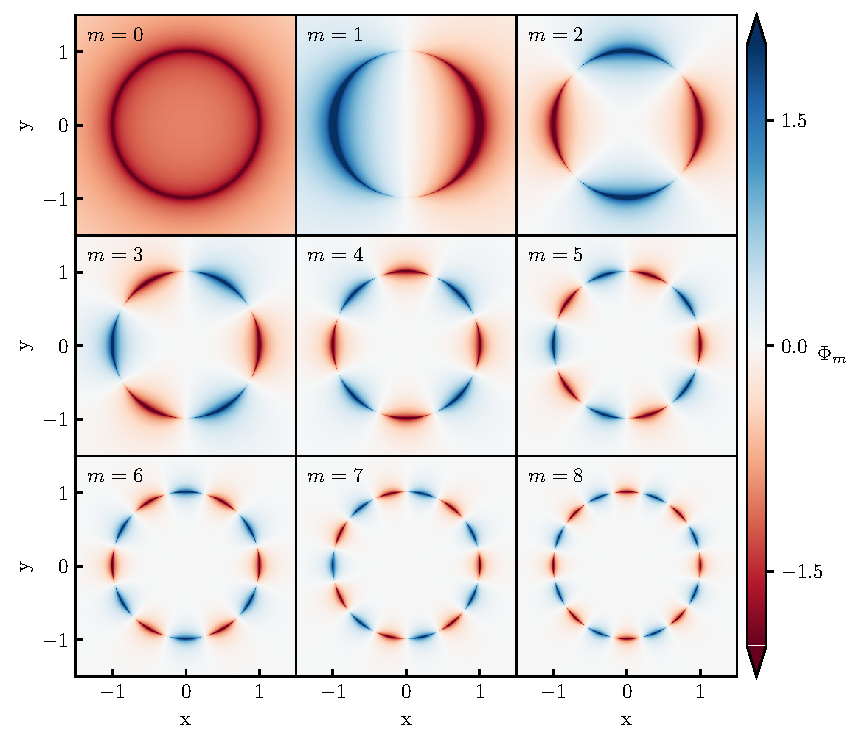
\includegraphics[width = 0.95\textwidth]{figures/planet_components.pdf}
    \caption{The first 9 Fourier components of the planet potential $\Phi_m(r,\phi) = V_m(r) \cos (m \phi)$, where the star is located at $(x,y) = (0,0)$ and the planet at $(1,0)$. The units are dimensionless such that $G=M_{\rm p}=1$. The Laplace coefficients $b_{1/2}^m$ were calculated using the \textsc{Python} package \textsc{PyLaplace} \citep{paardekooper2019a}}
    \label{fig:planet_fourier}
\end{figure}

From equation \ref{eq:fourier_planet} we find the following derivatives
\begin{align}
    \partial_r \Phi_m (r, \phi) &= \frac{dV_m(r)}{dr} \cos (m \phi) \\
    \partial_\phi \Phi_m (r, \phi) &= - m V_m(r) \sin (m \phi),
\end{align}
and so equation \ref{eq:lin_az_lindblad} becomes
\begin{align}
    \ddot{\phi} = - \frac{2 \Omega}{r} \dot{\delta r} + \frac{m V_m}{r^2} \sin \left( m [ \Omega - \Omega_{\rm p}] t\right),
\end{align}
and integrating gives
\begin{align}
    \dot{\phi} = - \frac{2 \Omega}{r} \delta r - \frac{V_m}{(\Omega - \Omega_{\rm p}) r^2} \cos \left( m [ \Omega - \Omega_{\rm p}] t \right).
\end{align}
Substituting this into \ref{eq:lin_rad_lindblad} yields
\begin{align}
    \ddot{\delta r} + \kappa^2 \delta r = \Psi_m(r) \cos (m [ \Omega - \Omega_{\rm p}] t), \label{eq:lindblad_forcing}
\end{align}
where
\begin{align}
    \kappa^2 \equiv \frac{d^2 \Phi_\star}{dr^2} + 3 \Omega^2 = r \frac{d \Omega^2}{dr} + 4 \Omega^2,
\end{align}
is the usual epicyclic frequency already introduced. In addition, we define the forcing function $\Psi_m(r)$ as
\begin{align}
    \Psi_m(r) \equiv - \left( \frac{dV_m}{dr}+ \frac{2 \Omega}{(\Omega - \Omega_{\rm p})r} V_m \right).
\end{align}
Equation \ref{eq:lindblad_forcing} is a second order, inhomogeneous differential equation in the form of a driven harmonic oscillator.
The general solution $g(t)$ is given by 
\begin{align}
    g(t) = A_1 \mathcal{H}(t) + A_2 \mathcal{P}(t),
\end{align}
where $\mathcal{H}(t)$ is the solution to the homogeneous equation where the right-hand side is zero, $\mathcal{P}(t)$ is a particular solution to the inhomogeneous equation, and $A_1$ and $A_2$ are the amplitudes of each.
Physically, $A_1 \mathcal{H}(t)$ corresponds to the ``free'' solution in the absence of forcing by the planet potential, and a non-zero value of $A_1$ results in particle orbits that are not closed.
$A_2 \mathcal{P}(t)$ corresponds to the driven solution and is what we are interested in here.
We solve for the driven solution using the ansatz $\delta r (t) = A \cos (m [\Omega - \Omega_{\rm p}]t)$, with the result that the amplitude of the response to the planet forcing is given by 
\begin{align}
    A = \frac{\Psi_m (r)}{\Delta_m},
\end{align}
where $\Delta_m$ is as defined in equation \ref{eq:def_delta_m}, and we have $\omega = m \Omega_{\rm p} $.
From this, we see that the forcing amplitude $A$ becomes very large as $\Delta_m \rightarrow 0$.
$\Delta_m = 0$ is therefore the condition for a \textit{Lindblad Resonance}; it determines the region where the response to periodic forcing by a particular component of the planet potential is greatest.
This is also the condition where the Lin-Shu dispersion relation breaks down as equations \ref{eq:lin_u_m} and \ref{eq:lin_v_m} become singular.

From equation \ref{eq:rotation}, we have that for material in a gas disk $\kappa = \Omega \approx \Omega_{\rm K}$.
Thus disk material is most effectively excited by the planet potential component $\Phi_m$ in the region where
\begin{align}
    \Omega_{\rm K}^2 = m^2 (\Omega_{\rm K} - \Omega_{\rm p})^2.
\end{align}
By substituting equation \ref{eq:point_pot} we obtain the \textit{Lindblad radii}
\begin{align}
    r_{\rm L}^\pm(m) = \left( 1 \pm \frac{1}{m} \right)^\frac{2}{3} r_{\rm p}, \label{eq:lind_loc}
\end{align}
which are the positions of the $m$th Lindblad resonances, where $r_{\rm L}^-$ is interior to the planets orbit and $r_{\rm L}^+$ is exterior to the planets orbit.
The Lindblad resonances are spatially segregated but become densely packed near $r_{\rm p}$ as $m$ becomes large, as shown in figure \ref{fig:lindblad}.
This segregation allows us to consider each resonance location as driven by only the $m$th component of the planet potential.
This breaks down for large $m$ as the resonances are no longer clearly separated.

The pressure support of the disk results in a slight modification of $\Omega$ from $\Omega_{\rm K}$ as seen in equation \ref{eq:rotation}.
This results in the radial shifting of the resonance positions \citep{artymowicz1993a}.
Resonance-shifting is important for calculating the total resultant torque on the disk, but affects the structure of excited waves only minimally and so we will ignore it here.

\begin{figure}
    \centering
    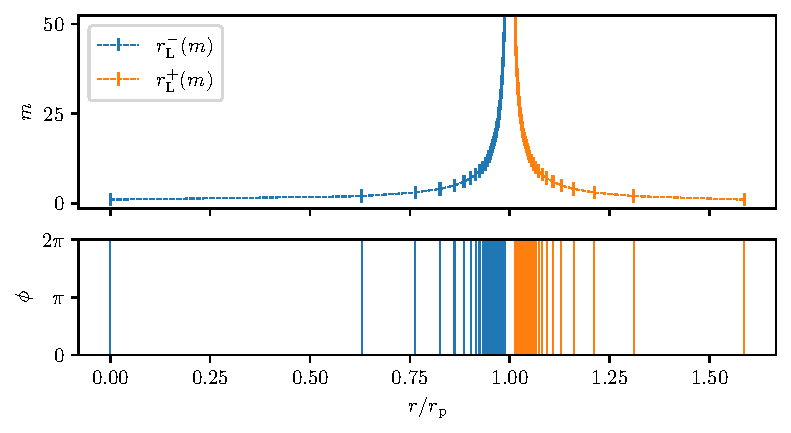
\includegraphics[width = 0.9\textwidth]{figures/lindblad_two_panel.pdf}
    \caption{Lindblad resonance positions as given by equation \ref{eq:lind_loc}. The bottom panel shows the physical radial locations in the disk where these resonances occur for different $m$, with the inner resonances coloured blue and the outer resonances coloured orange. The top panel shows how these position are related to $m$, and demonstrates the asymptotic behaviour of the resonance position $r_{\rm L}^\pm \rightarrow r_{\rm p}$ as $m \rightarrow \infty$.}
    \label{fig:lindblad}
\end{figure}

\subsection{The Planet Wake} \label{sec:planetwake}

Following closely the work by \citet{ogilvie2002}, we will use phase arguments to determine the shape of the planet wake in the linear density wave theory paradigm.
However we will not follow exactly their original derivation.
We will instead obtain the more general form for the wake shape.
Similarly to in section \ref{sec:linshu}, we can write linear wave quantities in a 2D gas disk as 
\begin{align}
    \delta a_m = A_m(r) \exp{i \Theta_m},
\end{align}
where the amplitude $A_m(r)$ varies slowly with radius and the phase
\begin{align}
    \Theta_m = \int^r k(r') \, dr' + m (\phi - \Omega_p t),
\end{align}
varies rapidly with radius. 
Again only the real component is physically relevant, and we have written $\omega = m \Omega_p$ as we are assuming the waves are generated by an embedded planet.
To investigate the shape of the spiral wake we will look for lines of constant phase that are defined by the condition $\frac{d\Theta_m}{dr} = 0$ and so 
\begin{align}
    \frac{d\phi}{dr} = - \frac{k}{m}. \label{eq:spiral_km}
\end{align}
This is the same as the relation used to find the pitch angle of the spiral shape in equation \ref{eq:pitchangle}.
Assuming Keplerian rotation such that $\kappa=\Omega=\Omega_{\rm K}$, we can find $k$ from the Lin-Shu Dispersion relation \ref{eq:lin_shu_disp}
\begin{align}
    k^2 &= \frac{m^2 \left( \Omega - \Omega_{\rm p} \right)^2 - \kappa^2}{c^2}, \\
    &= \frac{m^2 \Omega_{\rm K}^2}{c^2} \frac{1}{r_{\rm p}^3} \left[ r^{3/2} - \left( r_{\rm L}^+ \right)^{3/2} \right] \left[ r^{3/2} - \left( r_{\rm L}^- \right)^{3/2} \right].
\end{align}
The tidal forcing of the planet results in density waves launched at the Lindblad resonances, with those launched at $r_{\rm L}^-$ and $r_{\rm L}^+$ propagating inwards and outwards through the disk respectively \citep{goldreich1978,goldreich1979}.
Figure \ref{fig:wakes_m3} shows the shape of the $m=3$ spiral waves generated at the $r_{\rm L}^\pm (m=3)$ Lindblad resonances as they propagate away from the planet.
The shape of these spirals is calculated as follows.
\begin{figure}
    \centering
    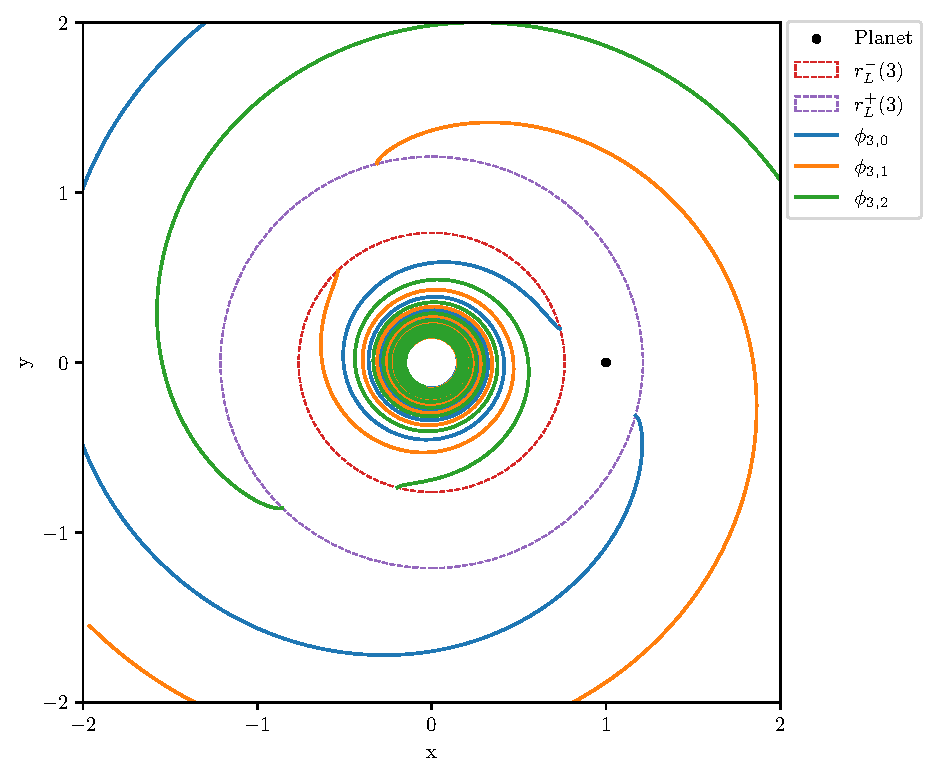
\includegraphics[width = 0.9\textwidth]{figures/wakes_m3.pdf}
    \caption{Schematic overview of the $m=3$ mode excited in a Keplerian disk. The disk has sound speed $c \propto r^{-1/4}$ where the aspect ratio at the planet is $(H/r)_{\rm p} = 0.1$.
    The planet is placed at $(1,0)$ and the inner and outer Lindblad resonances are shown by the red and purple dashed lines respectively.
    The blue, orange and green solid lines show lines of constant phase for the $n=0,1,2$ spiral arms excited at the resonances as they propagate inwards and outwards in the disk.
    These lines were calculated using equations \ref{eq:phase} -- \ref{eq:planet_wake}.}
    \label{fig:wakes_m3}
\end{figure}
Placing ourselves in the frame where the planet is stationary at $\phi = 0$, we can find the phase of the spiral waves simply by integrating equation \ref{eq:spiral_km} giving \citep{bae2018a}
\begin{align}
    \phi_m (r) = \phi_m(r_{\rm L}^\pm) - \int_{r_{\rm L}^\pm}^r \frac{k(r')}{m} \, dr', \label{eq:phase}
\end{align}
which consists of a constant offset $\phi_m(r_{\rm L}^\pm)$ term that gives the azimuthal launching location, plus a term that varies with radius.
For the waves launched at the Lindblad resonances, the constant offset term can be found from the asymptotic behaviour of the Airy function \citep{ward1986}. 
For the $n$th arm of the $mth$ mode, where $n = 0, 1, ..., m-1$ the offset is given by 
\begin{align}
    \phi_{m,n}(r_{\rm L}^\pm) = - \sign (r_{\rm L}^\pm - r_{\rm p}) \frac{\pi}{4m} + 2 \pi\frac{n}{m}. \label{eq:spiral_offset}
\end{align}
Now considering the $n=0$ arm, we see from the above that it launches closest to $\phi=0$ and thus closest to the planet.
For large $m$, we find that the constant offset term $\phi_{m,0}(r)$ becomes independent of $m$.
In addition, we have that $r_{\rm L}^\pm \rightarrow r_{\rm p}$ as $m \rightarrow \infty$.
This results in the formation of a coherent, one-armed spiral wave centred on the planet, as \ref{eq:phase} and \ref{eq:spiral_offset} reduces to
\begin{align}
    \phi_{\infty,0}(r) = - \int_{r_{\rm p}}^ r \frac{\Omega(r') - \Omega_{\rm p}}{c(r')} \, dr'. \label{eq:planet_wake}
\end{align}
Because the $n=0$ waves launch almost in phase nearby the planet, as seen in figure \ref{fig:planet_wake}, the planet wake is always centred on the planet location. 
The above result was first found by \citet{ogilvie2002}, although they wrote it in a different form. 
They dubbed the resultant spiral wave the planet ``wake'' in analogy with the Kelvin wedge produced by a ship moving through water.
The form shown above was first given in \citet{rafikov2002a}.

\begin{figure}
    \centering
    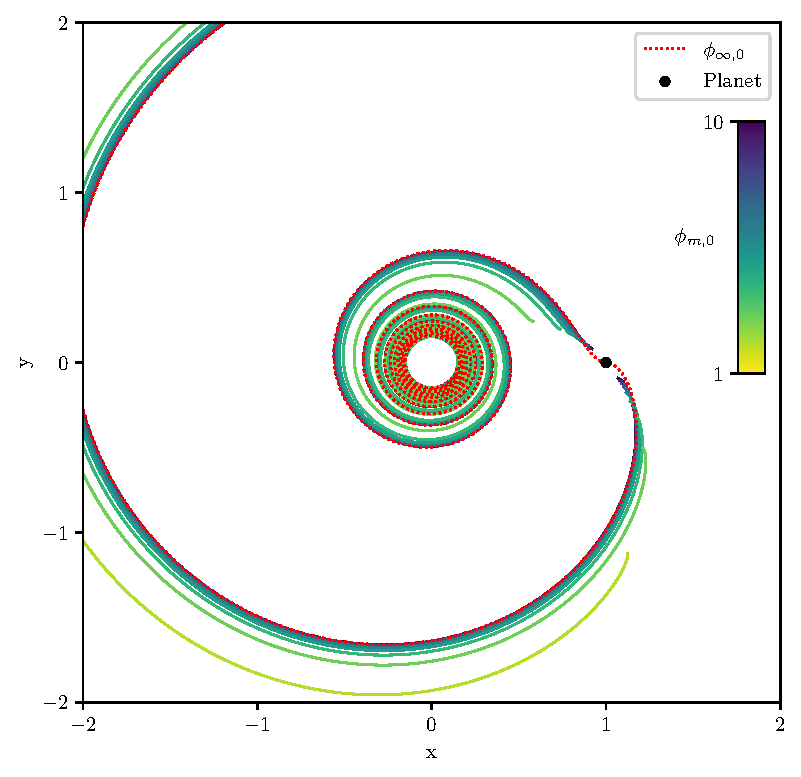
\includegraphics[width = 0.8\textwidth]{figures/planet_wake_shape.pdf}
    \caption{Plot of the $n=0$ spiral arms defined by the lines of constant phase $\phi_{m,0}$ for modes $m=1,...,10$ (solid lines).
    $\phi_{\infty,0}$ is shown with the red dotted line.
    The planet is placed at $(1,0)$ once again and the disk parameters are as in Figure \ref{fig:wakes_m3}.
    We see that asymptotically $\phi_{m,0}$ approaches the planet wake shape $\phi_{\infty,0}$ as the line of constant phase loses its $m$ dependence for large $m$.}
    \label{fig:planet_wake}
\end{figure}

Ogilvie and Lubow also investigated the degree to which the constructive interference along $\phi_{\infty,0}$ fails.
To do this they calculated the relative error $\Delta_m$ in the phase for each $m$ caused by the approximation we have performed above.
Note that this is not the same quantity as we defined in \ref{eq:def_delta_m}.
Figure \ref{fig:delta_m} shows $\Delta_m$ in both the outer and inner disk, for multiple values of $m$.
We see that in general, the approximation improves for larger $m$.
Additionally, the behaviour in the inner and outer disk is very different.
Ogilvie and Lubow found that $\Delta_m \sim \mathrm{constant}$ as $r \rightarrow \infty$, while $\Delta_m$ diverges as $r \rightarrow$ 0, and that for any fixed $r$, $\Delta_m \rightarrow 0$ as $m \rightarrow \infty$.
Thus the accuracy of the one-armed wake shape \ref{eq:planet_wake} is in general better in the outer disk than the inner disk, and also depends on the importance of each mode.
If the wave is dominated by large $m$ then \ref{eq:planet_wake} holds everywhere except for very small disk radii, while always failing if dominated by $m=1$ or $2$ \citep{ogilvie2002}.
The dominating azimuthal mode for tidal forcing by a planet is $m_{\rm D} \approx 1/2 \left( H/r \right)_{\rm p}^{-1}$ \citep{goldreich1980}, and so for observed protoplanetary disks $m_{\rm D} \gtrsim 5$ \citep{law2021a}. 
The coherent planet wake picture should therefore hold well except for at small disk radii.

\begin{figure}
    \centering
    \begin{subfigure}[b]{0.49\textwidth}
        \centering
        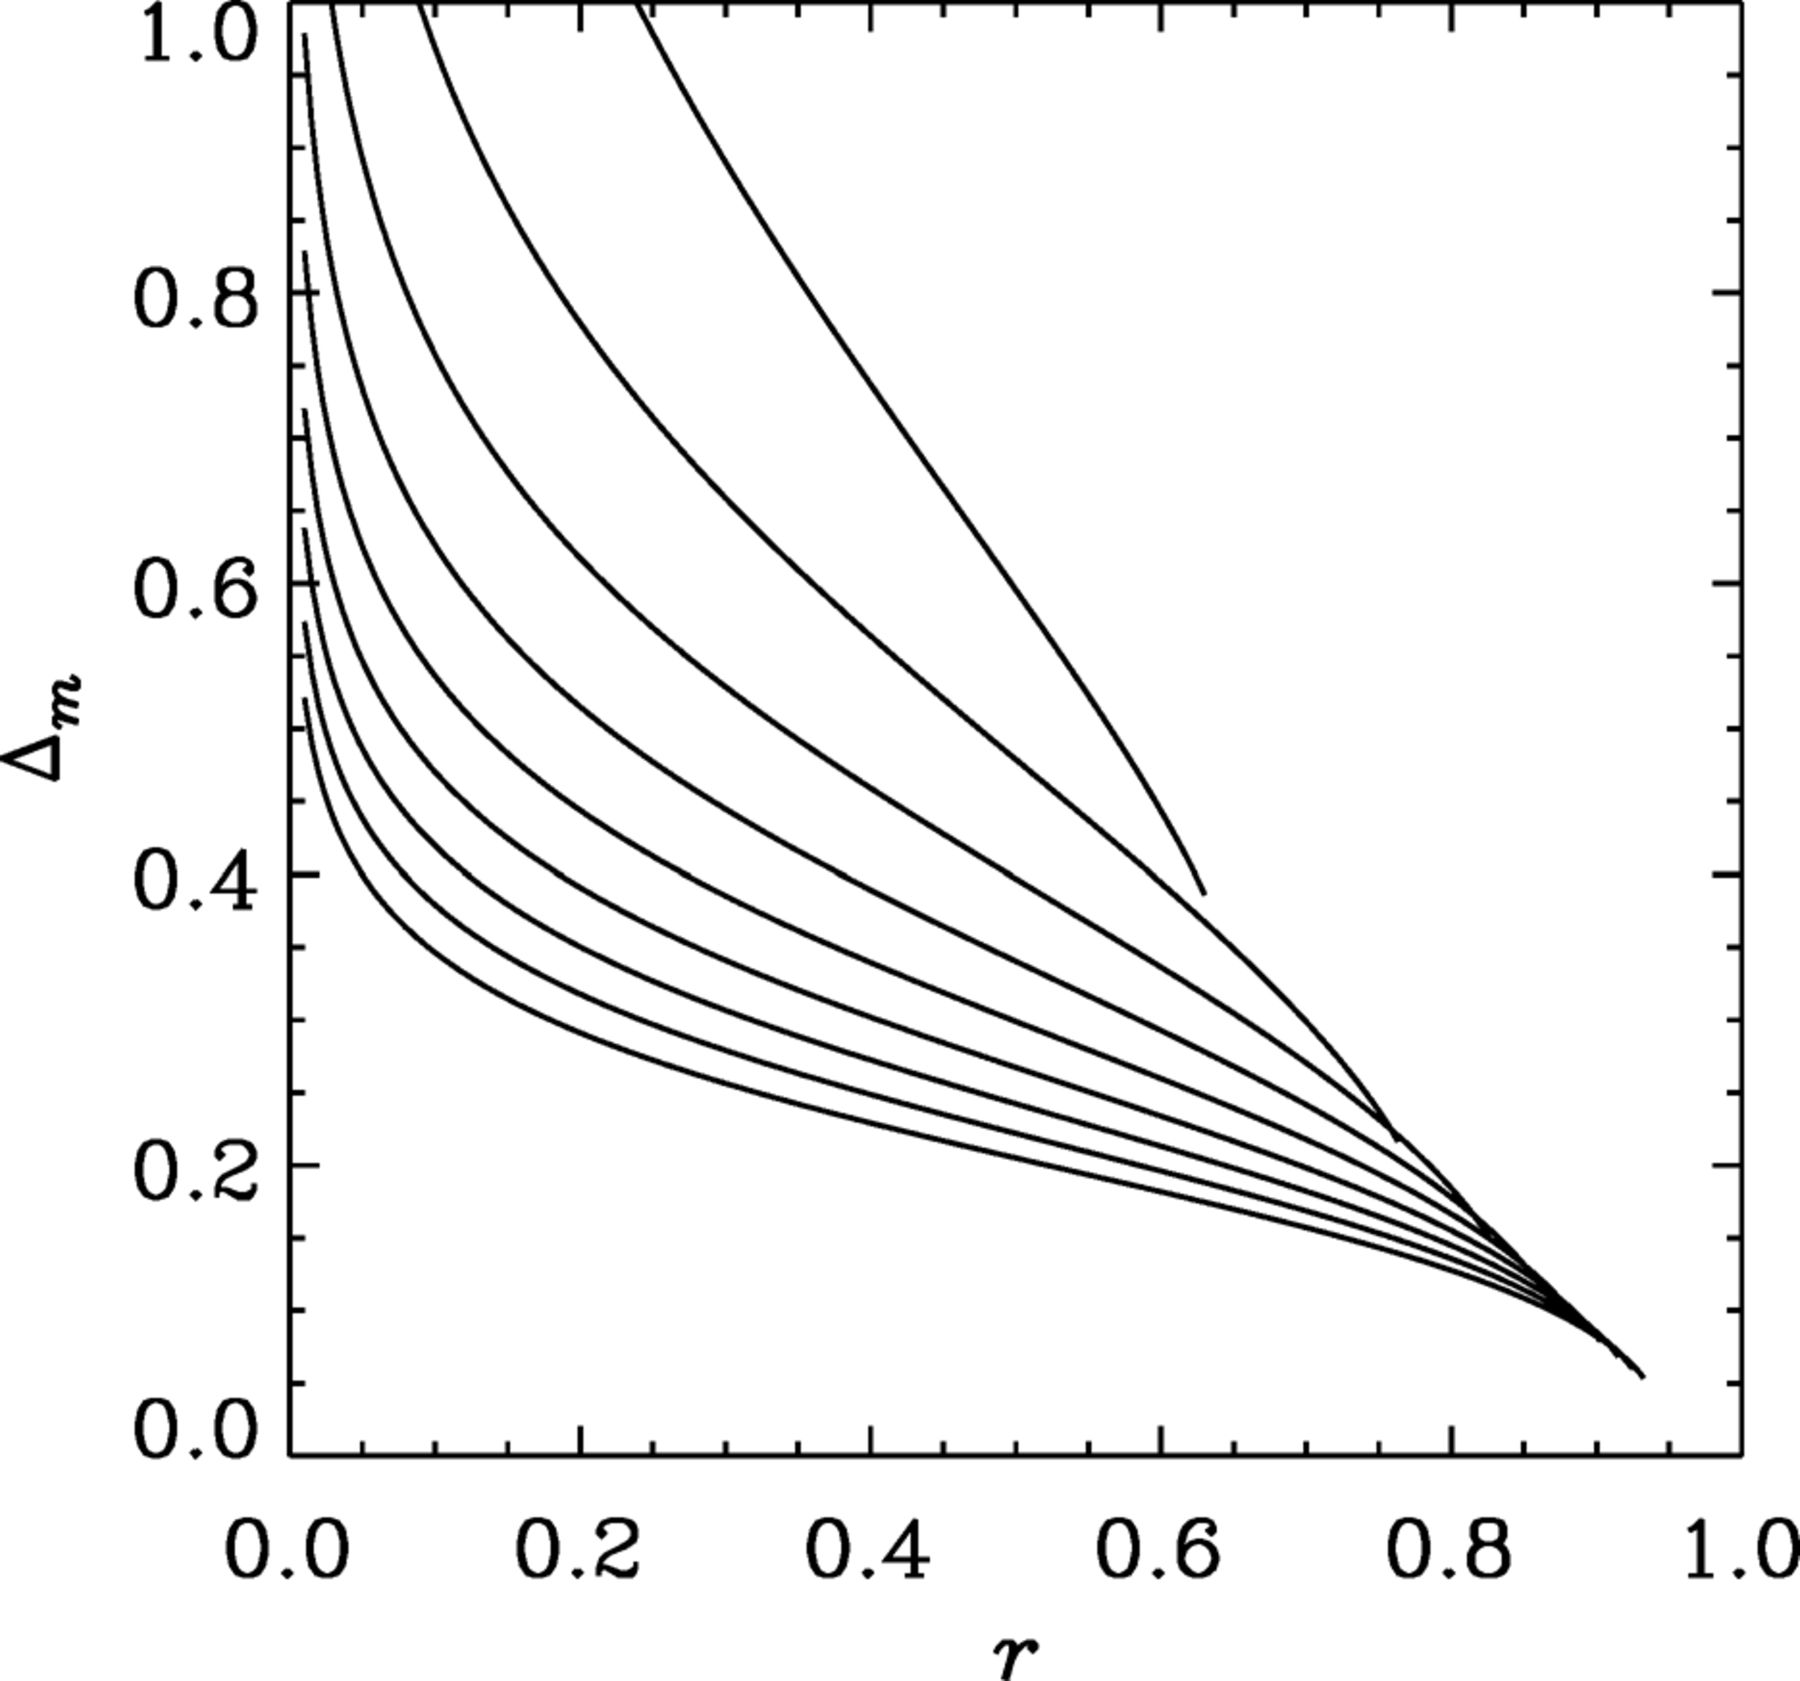
\includegraphics[width=\textwidth]{figures/Delta_m_inner.jpeg}
        %\caption{$y=x$}
        \label{fig:delta_m_inner}
    \end{subfigure}
    \hfill
    \begin{subfigure}[b]{0.49\textwidth}
        \centering
        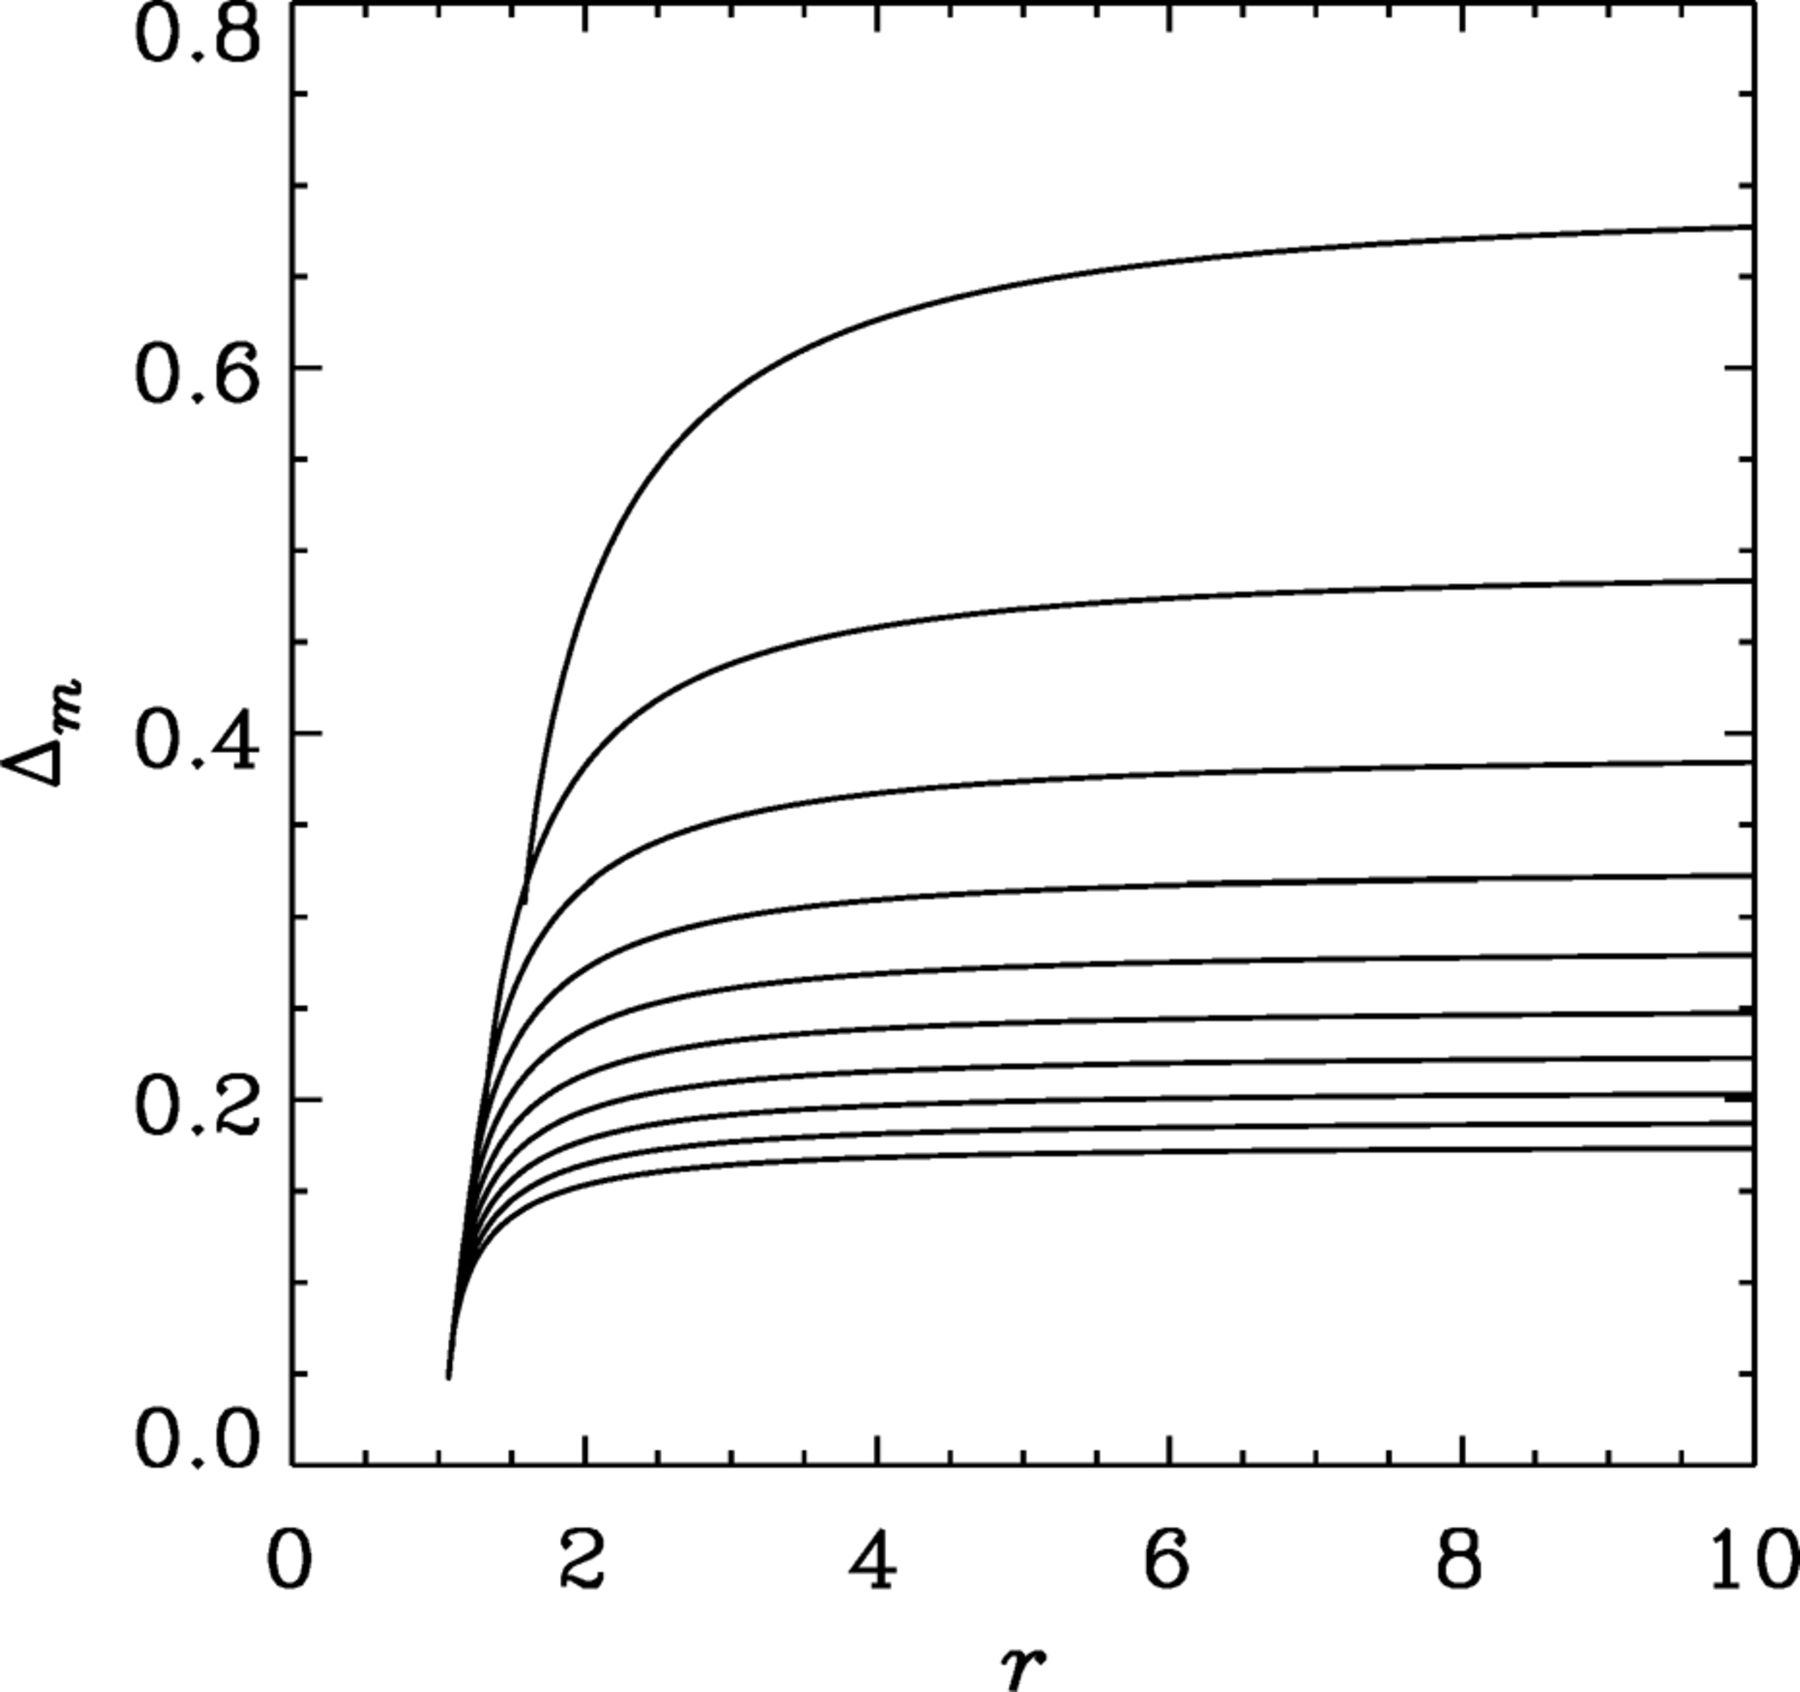
\includegraphics[width=\textwidth]{figures/Delta_m_outer.jpeg}
        %\caption{$y=3sinx$}
        \label{fig:delta_m_outer}
    \end{subfigure}
       \caption{The error in the phase $\Delta_m$ resulting from neglecting the $m$ dependence in equation \ref{eq:phase}, plotted for both the inner (left) and outer (right) disk \citep{ogilvie2002}.
       The planet is placed at $r=1$. Modes $m=1,...,10$ are shown from top to bottom.
       We see that the approximation improves for large $m$ as expected.}
       \label{fig:delta_m}
\end{figure}

\subsection{Additional Spiral Arms}

In addition to constructive interference of the $n=0$ components causing the planet wake, it is possible for additional spiral arms to form.
These \textit{secondary} and \textit{tertiary} spiral arms (where the planet wake described in the previous section is the \textit{primary} arm) were first seen in numerical calculations \citep{fung2015} and were not very well understood in the context of linear density wave theory until quite recently \citep{bae2018a,miranda2019a}.
Unlike the primary, these spirals are not centred on the planet position, and are instead generated some distance away in the inner disk.

Figure \ref{fig:additional_arms} shows the phase of the $n=1$ and $n=2$ components in the inner disk.
We see that unlike for the $n=0$ case, the waves are not launched in the vicinity of the planet, or nearby each other.
However the overall behaviour of the constant offset launching term \ref{eq:spiral_offset} is the same for non-zero $n$, namely that it becomes smaller as $m$ increases and so the launching phases become closer for larger $m$.
Furthermore, the modes become more tightly wound as $m$ increases, with the second term of \ref{eq:phase} also losing its $m$ dependence for very large values.
These effects allow the larger $m$ modes launched closer to the planet to catch up to the low $m$ modes.
\citet{bae2018a} first performed this analysis and proposed that this catching up effect is responsible for the generation of secondary and tertiary spirals.
This also provides a natural explanation as to why the additional arms are not centred on the planet, as the interference only becomes coherent after the large $m$ modes have caught up in phase.
Bae and Zhu also found that this effect does not operate in the outer disk, as the difference in phase between small and large $m$ modes becomes constant instead of decreasing.

\begin{figure}
    \centering
    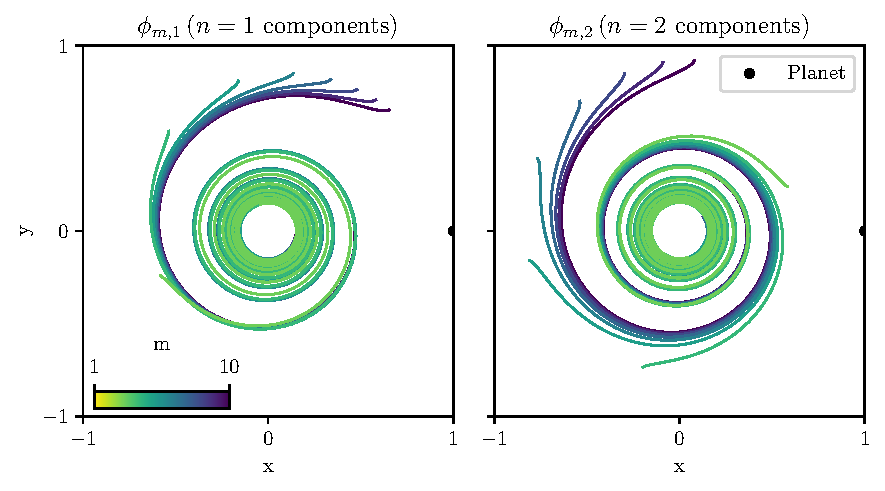
\includegraphics[width = 0.95\textwidth]{figures/inner_n_1_and_2.pdf}
    \caption{Plot of the $n=1$ (left) and $n=2$ spiral arms defined by $\phi_{m,n}$ for modes $m=1,...,10$ (solid lines).
    We show only the inner disk, with the planet placed at $(1,0)$ and disk parameters as in Figure \ref{fig:wakes_m3}.
    We see that in both the $n=1$ and $n=2$ case, although the spirals start initially out of phase due to different launching positions, the larger $m$ modes are able to catch-up resulting in the formation of the coherent secondary and tertiary spiral arms respectively.}
    \label{fig:additional_arms}
\end{figure}

\citet{miranda2019a} built upon this work through numerical calculations and showed that the formation of additional arms in the inner disk is a robust prediction of the linear theory.
They did this by taking into account the global mode structure outside of the WKB approximation as used in \citet{bae2018a}, and calculated both the phase and amplitude of each mode.
They found that their results in general supported the picture of additional arms resultant from coincident phases, but that taking into account the amplitude information changes the level of correspondence and can be important, especially for the tertiary and higher order arms (those formed by $n>2$).

In this work we will be concerned primarily with the waves generated by the planet in the outer disk and so our models will not include any of the additional arms in the inner disk, only the primary planet wake.

\section{Linear Planet Wake Excitation} \label{sec:linear_wake_excitation}

We now move on to calculating the density and velocity perturbations in the vicinity of the planet due to the planet wake.
This follows the method presented in \citet{goodman2001,rafikov2002a}, which itself is based on the seminal work by \citet{goldreich1978,goldreich1980}.
This involves calculating the linear disk response for each of the Fourier modes of the perturbations.
The solutions are \textit{global} since the WKB approximation is not used.
Historically the interest was first in calculating the Lindblad torque and not the profile of the wake itself, and so the phases of the Fourier harmonics were neglected \citep{goldreich1978,goldreich1980,artymowicz1993a,ward1997}.
\citet{goodman2001} included these phases to solve directly for the shape of the wake.
Their approach for calculating the wake structure splits the problem into two separate regimes: 
\begin{enumerate}
    \item Linear wake \textit{generation}: Provided that $M_{\rm p}$ is not too large ($\lesssim M_1$ defined in equation \ref{eq:char_mass}), the disturbance of the planet nearby the planet is weak enough that the wake can be calculated from linear theory.
    \item Non-linear wake \textit{propagation}: As the wave travels away from the planet it steepens into a shock and non-linear behaviour becomes important.  
\end{enumerate}
This approach is agnostic to the rotation, density and sound speed profiles of the disk, assuming only that they are functions of radius.
It is also assumed that the disk is locally polytropic (see section \ref{sec:velocity_perts}), inviscid, and non-self-gravitating.

It should be noted that the used of the language ``generation'' and ``propagation'' are slightly misleading.
The solution that we will calculate is mathematically a steady-state and has no time dependence.
In a physical sense the language is correct; waves are excited nearby the planet before propagating out into the disk.
In a mathematical sense the language is potentially confusing since the solution is independent of time.
These two opposing points of view are reconciled by considering that we are working in the frame where the planet is stationary. 
In reality the spiral pattern is \textit{not} stationary.
The remainder of this section is dedicated to outlining the linear wake generation, while the following section describes the non-linear propagation.

Above we stated that nearby the planet the disturbance is weak enough that linear theory is sufficient to describe wake generation provided the planet is not too large.
This certainly seems counter-intuitive at first glance, should the disturbance not be largest in the direct vicinity of the planet?
This is explained by the fact that a stationary perturber cannot excite density waves in a subsonic flow \citep{landau1959}.
Thus no waves are generated within some characteristic distance from the planet, an effect known as the \textit{torque cut-off} \citep{goldreich1980}.
In a Keplerian disk this distance is $2H_{\rm p}/3$.
The Lindblad resonances within this region, where $m$ is large, are suppressed and therefore contribute minimally to the torque.
In addition the resonances with very low $m$ are not effectively excited due to their distance from the planet.
Indeed the dominant mode is of order $(H_{\rm p} / r_{\rm p})^{-1}$, as mentioned in section \ref{sec:planetwake}.
The resonances excited most efficiently are therefore located a few $H_{\rm p}$ from the planet, far enough to justify the linear approach.

\begin{figure}
    \centering
    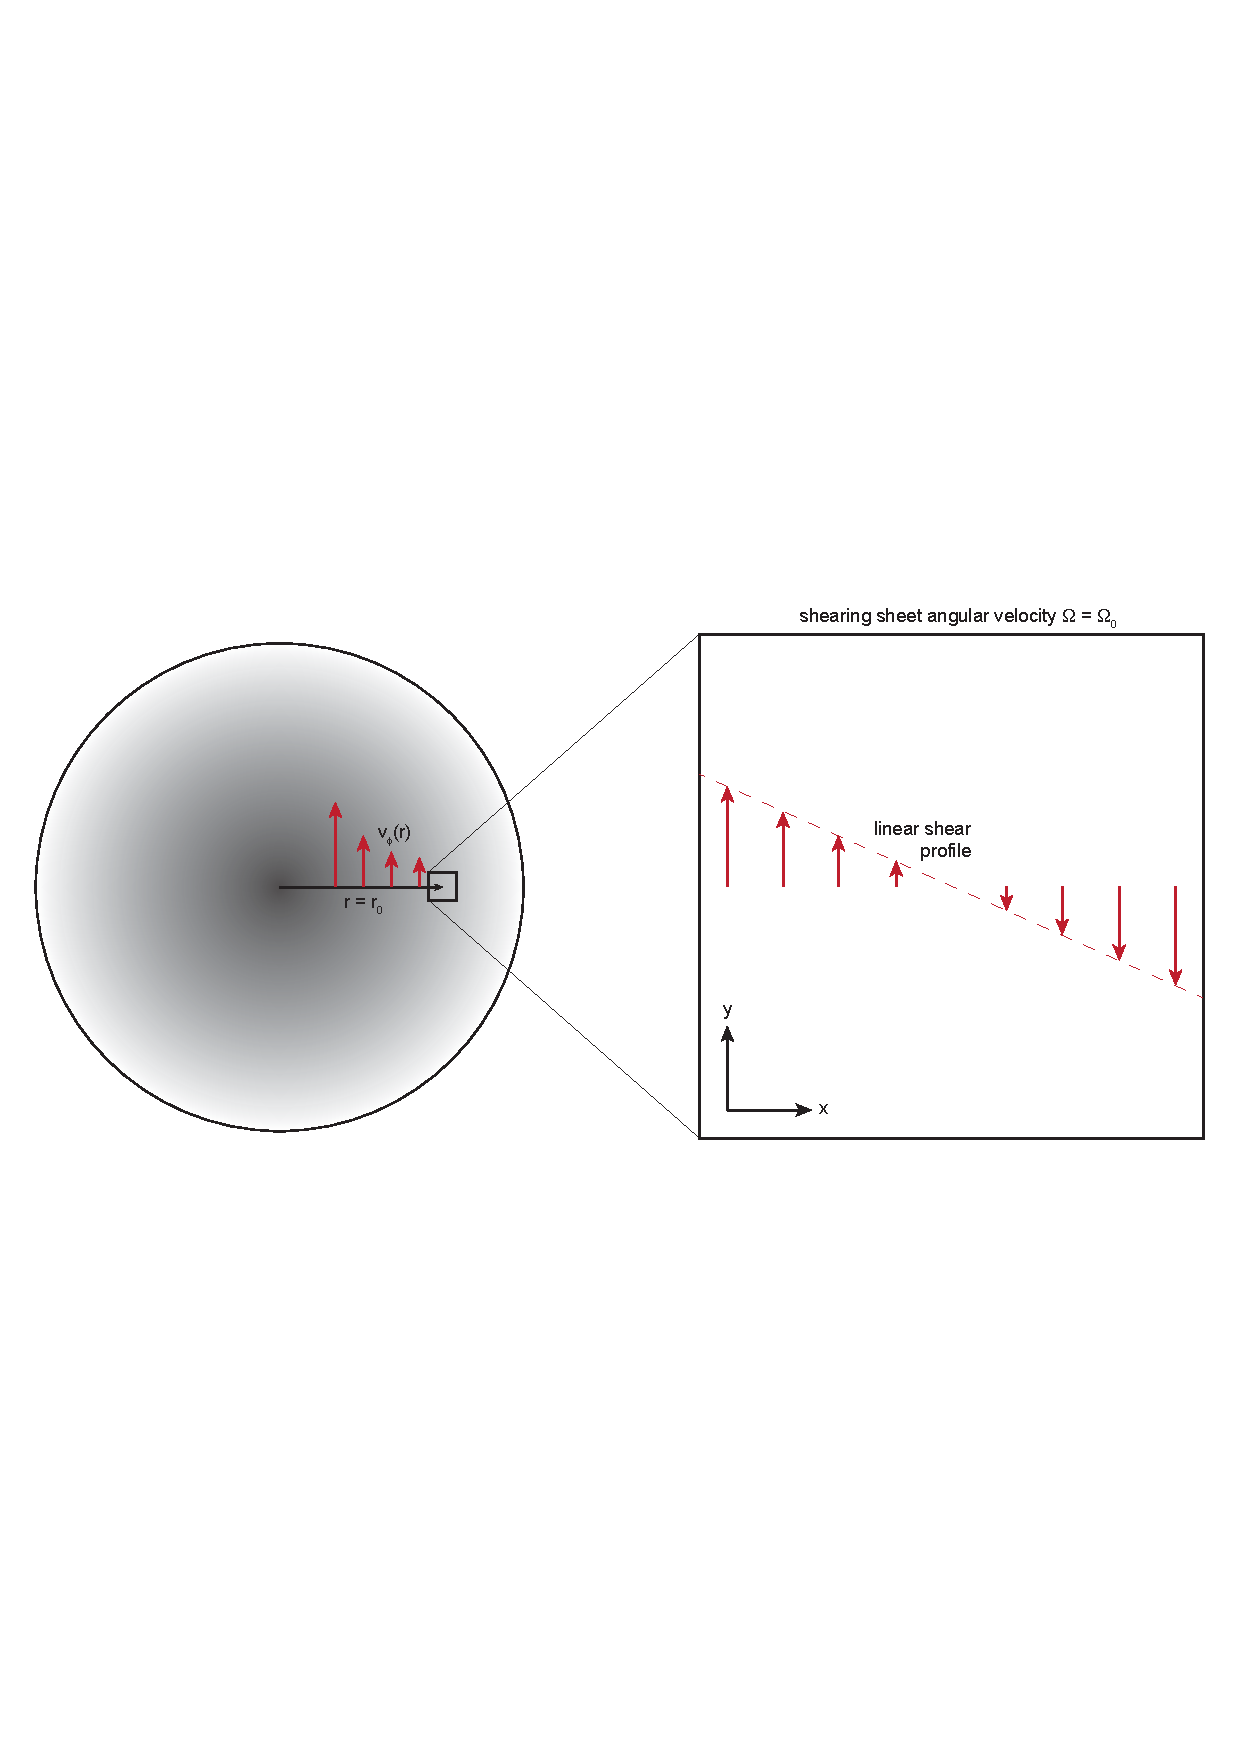
\includegraphics[width = 0.95\textwidth]{figures/shearing_sheet.pdf}
    \caption{Schematic diagram of the sheared-sheet approximation from the lectures notes by \citet{armitage2022}, where in our case $r_0 = r_{\rm p}$ and $\Omega_0 = \Omega_{\rm p}$ and so the shearing box is centred on the planet location.
    Under the approximation the shear nearby the planet is taken to be linear, while the surface density and sound speed are taken to be constant.}
    \label{fig:sheared_sheet}
\end{figure}

The rest of this subsection directly follows \citet{goodman2001}. 
The linear calculation is performed in the \textit{sheared-sheet approximation} \citep{hill1878,goldreich1965}.
This involves defining pseudo-cartesian coordinates centred on the planet location
\begin{align}
    x &= r - r_{\rm p}, \\
    y &= r_{\rm p} \left( \phi - \phi_{\rm p} \right),
\end{align}
where $\phi_{\rm p}$ is the azimuthal location of the planet.
The differential rotation of the disk is then expanded to lowest order in $x/r_{\rm p}$, which reduces the azimuthal component of the flow to
\begin{align}
    v_0 = 2 A x; \qquad 2A \equiv r \left. \frac{d \Omega}{dr} \right|_{r_{\rm p}},
\end{align}
where the shear $A$ and rotation $\Omega$ rates are treated as constant (that does \textit{not} make the above derivative zero), as is the vorticity $B \equiv A+\Omega$.
The unperturbed surface density $\Sigma_{\rm p}$ and sound speed $c_{\rm p}$ are also assumed to be constant.
A diagrammatic overview of the sheared-sheet approximation is presented in Figure \ref{fig:sheared_sheet}.

We adopt as a length unit the mach-1 length $l_{\rm p}$, which is the distance from the planet where the flow becomes supersonic.
This requires that $v_0 = 2|Ax| > c_{\rm p}$ and so 
\begin{align}
    l_{\rm p} \equiv c_{\rm p} / |2A|. \label{eq:mach1_len}
\end{align}
For the planet mass we adopt the unit
\begin{align}
    M_1 \equiv \frac{c_0^3}{|2A|G}. \label{eq:char_mass}
\end{align}
For a Keplerian disk $M_1$ is equal to the \textit{thermal mass} defined in equation \ref{eq:thermalmass}.
For $M_{\rm p} \gtrsim M_1$ the Roche lobe of the planet will become larger than $l_{\rm p}$, causing the linear approximation to fail.
This is also the gap opening condition for an inviscid disk as discussed in section \ref{sec:gap_opening}.
In the linear regime the amplitude of the wake is directly proportional to the planet mass, and so it is sufficient to carry out the calculation only once and scale it appropriately as needed.

In the frame of the planet the wake is stationary such that the radial velocity, azimuthal velocity and density perturbations, $u, v$ and $\sigma = \delta \Sigma / \Sigma$ respectively, are independent of time.
The spatial Fourier transform of these components $\hat{u}, \hat{v}, \hat{\sigma}$ are functions of the coordinate wavenumbers $k_x$ and $k_y$, and they satisfy \citep{goldreich1978,goldreich1980}
\begin{align}
    \frac{d^2 \hat{v}}{d \tau^2} + \left[ c^2 k^2 + \kappa^2 \right]\hat{v} &= -i k_y \frac{d \hat{\Phi}_{\rm p}}{d\tau} + 2i k_x B \hat{\Phi}_{\rm p} \\
    \hat{u} &= - \frac{1}{c^2 k_y^2 + 4 B^2} \left( 2 B \frac{d \hat{v}}{d\tau} - c^2 k_x k_y \hat{v} + 2iBk_y \hat{\Phi}_{\rm p} \right) \\
    \hat{\sigma} &= \frac{i}{c^2 k_y^2 + 4 B^2} \left( k_y \frac{d \hat{v}}{d \tau} + 2B k_x \hat{v} + i k_y^2 \hat{\Phi}_{\rm p} \right),
\end{align}
where
\begin{align}
    \tau \equiv -\frac{k_x}{2 A k_y},
\end{align}
is a pseudo-time variable, $k=\sqrt{k_x^2 + k_y^2}$ is the instantaneous wavenumber, and $\hat{\Phi}_{\rm p}=-2\pi G M_{\rm p} / k$ is the Fourier transform of the planet potential.
This system of ordinary differential equations, combined with the initial condition that $\hat{v}=0$ as $\tau \rightarrow - \infty$, constitute a determined system where the unique solution provides the density and velocity perturbations along the wake after Fourier transforming back to coordinate space.

\section{Non-Linear Planet Wake Evolution} \label{sec:nonlinear_evolution}

\citet{goodman2001} first studied the non-linear evolution of the planet wake, neglecting both the disk geometry and variations in density and sound speed, while \citet{rafikov2002a} updated the analysis to include these effects.
We are obviously interested in accounting for these aspects and so we will largely follow \citet{rafikov2002a} in this section, but we will endeavour to make it clear when a result is originally from \citet{goodman2001}.

After the wake is generated, it propagates away from the planet.
At distances $\gg l$ the contribution of the planet potential becomes negligible.
However unlike in the sheared sheet, we must now consider the evolution of $\Sigma$ and $c$ with radius, as well as the global geometry of the disk.
Rewriting the 2D inviscid fluid equations \ref{eq:mom_eq_u}-\ref{eq:cont_2d} in a rotating frame such that the planet is stationary at $\phi=\phi_{\rm p}$, and $\phi$ is defined such that $\Omega>0$, we obtain \citep{landau1959}
\begin{align}
    &v_r \partial_r v_r + \frac{v_\phi}{r} \partial_\phi v_r - \frac{v_\phi^2}{r} = - \partial_r \Phi - \frac{1}{\Sigma} \partial_r P + 2 \Omega_{\rm p} v_\phi + \Omega_{\rm p}^2 r, \label{eq:mom_eq_u_pl} \\ 
    &v_r \partial_r v_\phi + \frac{v}{r} \partial_\phi v_\phi - \frac{v_r v_\phi}{r} = - \frac{1}{r} \partial_\phi \Phi - \frac{1}{r\Sigma} \partial_\phi P - 2 \Omega_{\rm p} v_r, \label{eq:mom_eq_v_pl} \\
    &\frac{1}{r} \partial_r (r \Sigma v_r) + \frac{1}{r} \partial_\phi (\Sigma v_\phi) = 0,
    \label{eq:cont_2d_pl}
\end{align}
where we have also dropped all time dependence, and $\Phi=\Phi_\star$ since we are neglecting the planet potential.

We now perform a perturbative study including weak non-linear behaviour.
We rewrite the velocities as 
\begin{align}
    v_r = u; \quad v_\phi = v_0(r) + v,
\end{align}
where
\begin{align}
    v_0(r) = r \Delta \Omega \equiv r \left( \Omega - \Omega_{\rm p} \right).
\end{align}
$u$ and $v$ are thus the radial and azimuthal velocity perturbations.
We assume that the shock formed is weak (we will refer to this as the \textit{weak shock approximation}) such that $|u|,|v| \ll |v_0|$. 
$\Delta \Omega \neq 0$ since we are working in region away from the planet.
In addition, the WKB approximation is applied such that $v \ll u$ and $\partial_\phi \ll r \partial_r$ as shown in the appendix of \citet{rafikov2002a}.
With the above considerations, equations \ref{eq:mom_eq_u_pl} - \ref{eq:cont_2d_pl} are transformed to 
\begin{align}
    &\Delta \Omega \partial_\phi u + u \partial_r u - 2 \Omega v = - \frac{1}{\Sigma} \left( \partial_r P - \partial_r P_0  \right) + \frac{v^2}{r}, \label{eq:weak_pert_1} \\
    &\Delta \Omega \partial_\phi v + u \partial_r v + 2Bu = - \frac{1}{r} \left( \frac{1}{\Sigma} \partial_\phi P +u v \right), \label{eq:weak_pert_2} \\
    &\Delta \Omega \partial_\phi \Sigma + u \partial_r \Sigma + \Sigma \partial_r u = - \frac{1}{r} \left( \Sigma u + v \partial_\phi \Sigma + \Sigma \partial_\phi v \right). \label{eq:weak_pert_3}
\end{align}
We have kept terms up to second order in $u$ and $v$.
The radial coordinate $\xi$ is now introduced, consisting of an integral transformation that essential encodes the differential rotation of the disk and simplifies the spatial propagation of the wake (note the similarity to equation \ref{eq:planet_wake}).
It is defined by
\begin{align}
    \xi = \int_{r_{\rm p}}^ r \left[ \Omega(r') - \Omega_{\rm p} \right] \, dr',
\end{align}
and results in the transformation of the equations \ref{eq:weak_pert_1} - \ref{eq:weak_pert_3} to
\begin{align}
    &\partial_\phi u + u \partial_\xi u + \frac{1}{\Sigma} \partial_\xi P - \frac{1}{\Sigma_0} \partial_\xi P_0 = \frac{1}{\Delta \Omega r} \left( 2 \Omega r v + v^2 \right), \label{eq:phi_xi_u} \\
    &\partial_\phi v + u \partial_\xi v + \frac{c^2}{\Delta \Omega r \Sigma} \partial_\phi \Sigma = - \frac{1}{\Delta \Omega r} \left( 2 B r u +uv \right), \label{eq:phi_xi_v} \\
    &\partial_\phi \Sigma + u \partial_\xi \Sigma + \Sigma \partial_\xi u = -\frac{1}{\Delta \Omega r} \left( \Sigma u + v \partial_\phi \Sigma + \Sigma \partial_\phi v \right). \label{eq:phi_xi_sigma}
\end{align}
The left-hand side of the equations above are similar to the usual system of equations that describe the motion of a one-dimensional isentropic gas \citep{landau1959}, except that we have an azimuthal coordinate $\phi$ in place of the time coordinate $t$ and the $\xi$ coordinate in place of the spatial coordinate $x$.
We exploit this similarity to simplify the above equations using the \textit{method of characteristics}.
the 1D isentropic gas flow system possesses two \textit{Riemann invariants} that are each conserved along a curve in the $xt$ plane.
These curves are called the \textit{characteristics}.
This is reviewed briefly in appendix \ref{appendix:isentropic_riemann}.
In our case the non-zero right-hand sides of the equations causes the Riemann invariants $R_\pm$ to no longer be conserved exactly along each of the characteristics $C_\pm$.
Instead, $R_\pm$ evolve in a predictable manner.
Following similar analysis to that in appendix \ref{appendix:isentropic_riemann}, we find that equations \ref{eq:phi_xi_u} and \ref{eq:phi_xi_sigma} reduce to 
\begin{align}
    \begin{split}
        \left[ \partial_\phi + (u \pm c) \partial_\xi \right] R_\pm = - &\left( \frac{1}{\Sigma} \partial_\xi P - \frac{1}{\Sigma_0} \partial_\xi P_0 - c\partial_\xi \frac{2c}{\gamma-1} \pm cu \frac{\partial_\xi \Sigma}{\Sigma} \mp u \partial_\xi \frac{2c}{\gamma-1} \right) \\
        &+ \frac{1}{\Delta \Omega r} \left( 2\Omega r v + v^2 \mp cu \mp cv \partial_\phi \ln \Sigma \mp c \partial_\phi v \right),
    \end{split}
\end{align}
where the Riemann invariants are
\begin{align}
    R_\pm = u \pm \frac{2c}{\gamma-1},
\end{align}
and the characteristics are
\begin{align}
    C_\pm : \, \frac{d\xi}{d\phi} = u \pm c.
\end{align}
The $C_-$ characteristic follows the planet wake, while the $C_+$ characteristic crosses it \citep{goodman2001}.
Therefore $C_-$ is always in the perturbed region while $C_+$ is predominantly in the unperturbed region.
By assuming that the wake-crossings affect the value of $R_+$ minimally and approximating its value as constant, we find that
\begin{align}
    R_+ = \frac{2 c_0}{\gamma - 1},
\end{align}
everywhere.
Since we are assuming $R_+$ is exactly conserved, this implies
\begin{align}
    u = \frac{2(c_0 - c)}{\gamma -1},
\end{align}
and so 
\begin{align}
    R_- = \frac{2(c_0 - 2c)}{\gamma -1}.
\end{align}
Based on these results it is possible to show that the system further reduces to a simple partial differential equation, the inviscid Burger's equation \citep[see appendix A of][]{rafikov2002a}
\begin{align}
    \partial_t \chi - \chi \partial_\eta \chi = 0, \label{eq:burgers}
\end{align}
where $\chi$ is a remapping of the surface density perturbation defined as 
\begin{align}
    \chi &\equiv \frac{\gamma +1}{2} \frac{\Sigma - \Sigma_0}{\Sigma_0} g(r), \label{eq:chi} \\
    {\rm where} \quad g(r) &\equiv \frac{2^{1/4}}{r_{\rm p} c_{\rm p} \Sigma_{\rm p}^{1/2}} \sqrt{\frac{r \Sigma_0 c_0^3}{|\Omega - \Omega_{\rm p}|}}, \label{eq:g}
\end{align}
and the coordinates $t$ and $\eta$ are defined as
\begin{align}
    t(r) &\equiv - \frac{r_{\rm p}}{l_{\rm p}} \int_{r_{\rm p}}^r \frac{\Omega(r') - \Omega_{\rm p}}{c_0(r') g(r')} \, dr', \label{eq:t} \\
    \eta(r,\phi) &\equiv \frac{r_{\rm p}}{l_{\rm p}} \left( \phi - \phi_{\rm p} + \int_{r_{\rm p}}^r \frac{\Omega(r') - \Omega_{\rm p}}{c_0(r')} \, dr'  \right) \label{eq:eta}
\end{align}
where $l_{\rm p}$ is the mach-1 length \ref{eq:mach1_len} and $\phi_{\rm p}$ is the azimuthal coordinate of the planet.
The $\eta$ coordinate can be written in a clearer form by comparing the third term with equation \ref{eq:planet_wake}:
\begin{align}
    \eta(r,\phi) &\equiv \frac{r_{\rm p}}{l_{\rm p}} \left( \phi - \phi_{\rm wake} \right), \\
    \rm{where} \quad \phi_{\rm wake} &\equiv \phi_{\rm p} - \int_{r_{\rm p}}^r \frac{\Omega(r') - \Omega_{\rm p}}{c_0(r')} dr'. \label{eq:phi_wake}
\end{align}
Intuitively, $t$ can be thought of a coordinate that travels \textit{along} the wake, while $\eta$ is a rescaled angular coordinate that \textit{crosses} the wake.
%To interpret these results we compare the characteristics with the planet wake.
%If we place the planet in our coordinates at azimuth $\phi_{\rm p}$, then from \ref{eq:planet_wake} the wake shape is given by 
%\begin{align}
%    \phi_{\rm wake} = \phi_{\rm p} - \int_{r_{\rm p}}^r \frac{\Omega(r') - \Omega_{\rm p}}{c_0(r')} \, dr'. \label{eq:wake_shape_rafikov}
%\end{align}
%In terms of $\xi$ this becomes
%\begin{align}
%    \phi_{\rm wake} &= \phi_{\rm p} - \int_{0}^\xi \frac{1}{c_0(\xi')} \, d\xi', \\
%    \Rightarrow \left. \frac{d \xi}{d \phi} \right|_{\rm wake} &= -c_0,
%\end{align}
%and so we see that $C_-$ follows the wake while $C_+$ crosses it.

\subsection{Wave Dissipation}

Burger's equation generically produces shocks from smooth waveforms due to the crossing of characteristics \citep{whitham1999}.
Figure \ref{fig:wake_profiles_GR01} shows the evolution of the wave profile taken at different $t$ values.
We see that at the edge of the linear regime the waveform is initially smooth.
As the wake evolves away from the planet its amplitude decays but areas above and below $\chi=0$ steepen and form two shocks, one moving in the $+\eta$ direction and one moving in the $-\eta$ direction.
The resultant waveform is called an \textit{N-wave} \citep{landau1959}.
\citet{goodman2001} found numerically that the shock forms at 
\begin{align}
    t_{\rm shock} = t_0 + 0.79 \left( \frac{M_{\rm p}}{M_1} \right)^{-1},
\end{align}
and so more massive planets produce a shock closer to the planet.

\begin{figure}
    \centering
    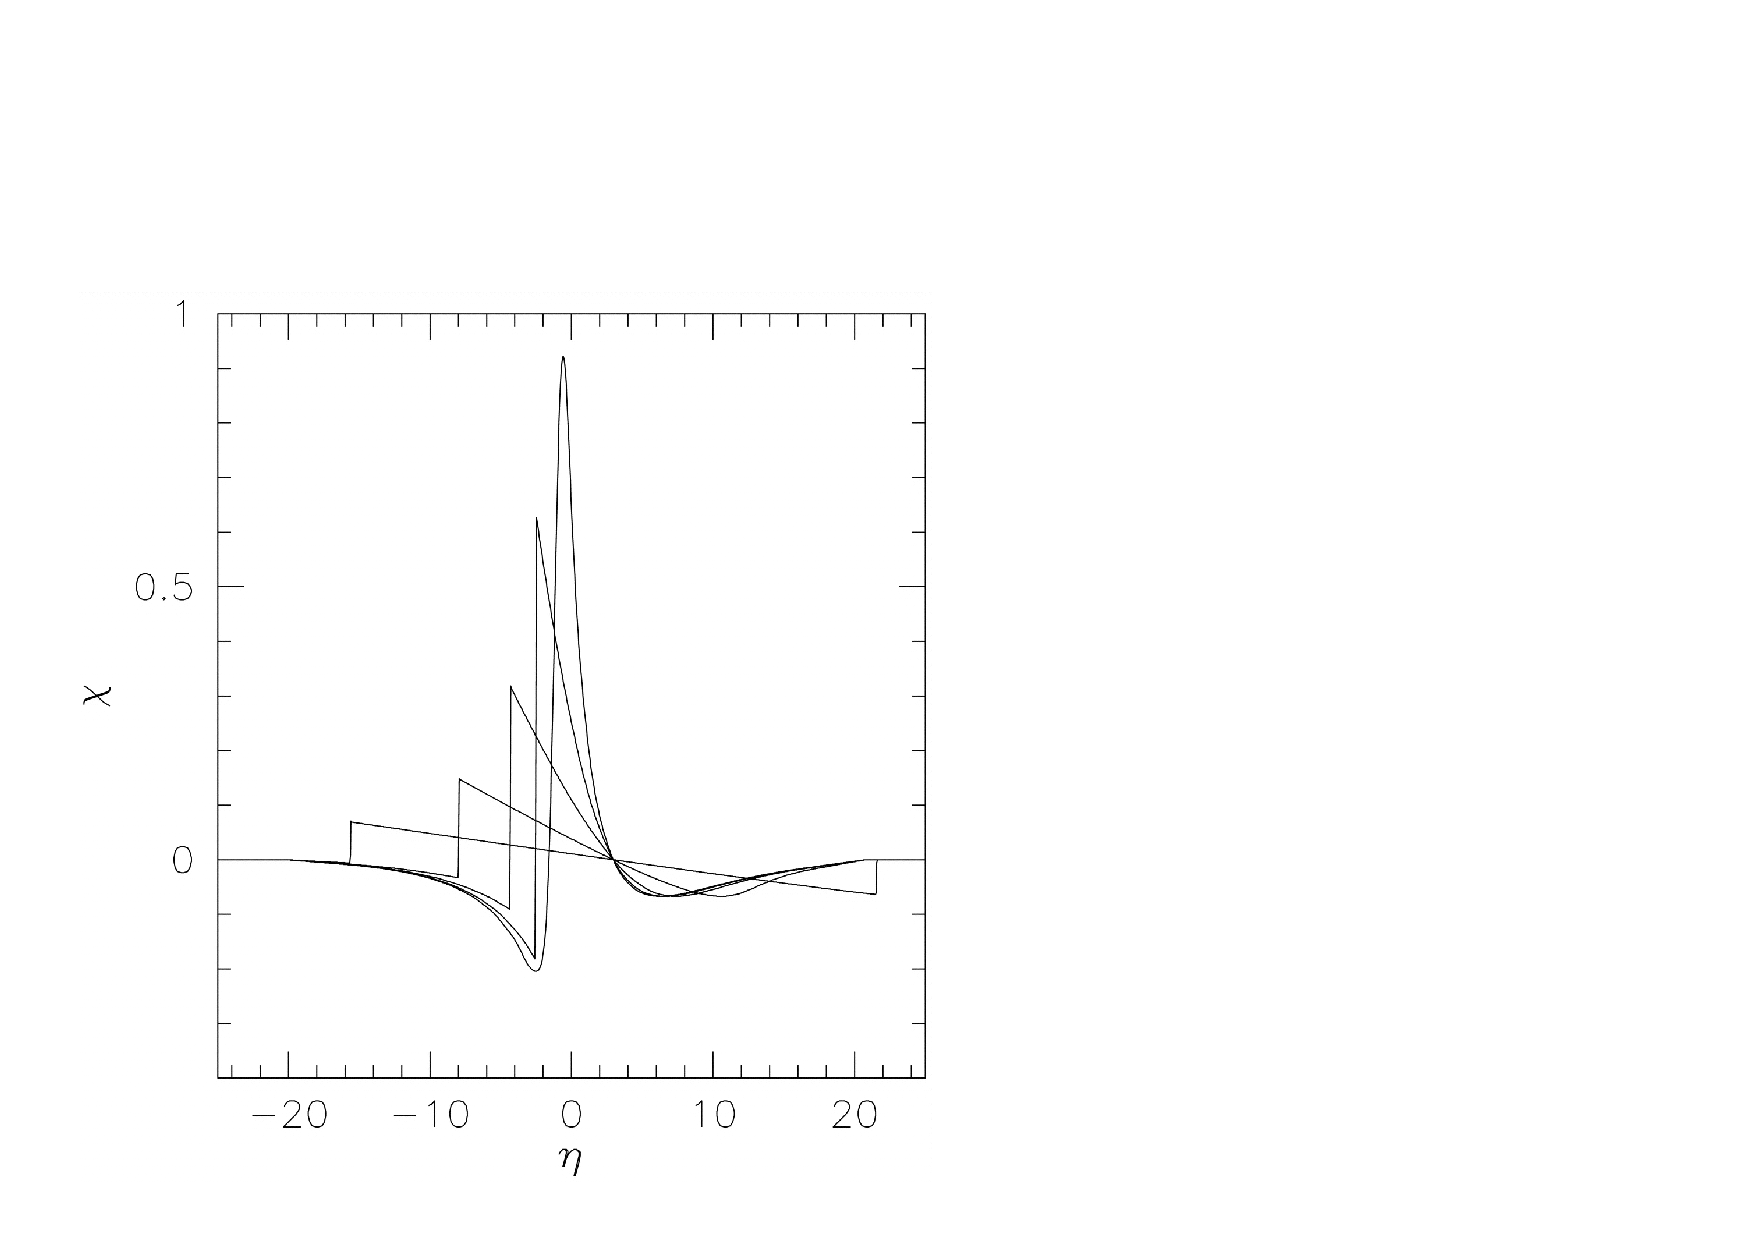
\includegraphics[width = 0.55\textwidth]{figures/wake_profiles_GR01.pdf}
    \caption{Evolution of the wake profile under the Burger's equation \ref{eq:burgers} from \citet{goodman2001}.
    They solved the equation using a second order advection scheme with initial conditions taken from the linear regime at a distance of 2$l_{\rm p}$ from the planet, corresponding to $t=t_0$.
    $\chi$ profiles are shown as slices in $t$ and as a function of $\eta$.
    These profiles were taken at $t-t_0 = 0, 4, 16, 64, 256$ in order of greatest to lowest amplitude.}
    \label{fig:wake_profiles_GR01}
\end{figure}

After the shock is formed the wave becomes dissipative;
its amplitude begins to decay as angular momentum is deposited into the disk.
Prior to shock formation the \textit{angular momentum flux} (AMF), the amount of angular momentum transported along the wake, is perfectly conserved.
The AMF $f_J$ can be calculated as \citep{rafikov2002a}
\begin{align}
    f_J(r) = \frac{c_0^3(r) r}{\Delta\Omega(r)\Sigma_0(r)} \int_0^{2\pi} \left( \Sigma - \Sigma_0 \right)^2 \, d\phi,
\end{align}
which we can rewrite as a function of $t$ using the transformations \ref{eq:chi}-\ref{eq:eta} giving
\begin{align}
    f_J(t) &= \frac{2^{3/2} c_{\rm p}^3 r_{\rm p} \Sigma_{\rm p}}{(\gamma + 1)^2 |2 A(r_{\rm p})|} \Phi(t), \\
    \rm{where} \quad \Phi(t) &= \oint \chi^2(t,\eta) \, d\eta 
\end{align}
is the dimensionless AMF, which we will always write as a function of $t$ to avoid confusion with the potential.
After shock formation the resultant dissipation results in the non-conservation of the AMF, as shown in figure \ref{fig:AMF}.

Recently \citet{cimerman2021} performed a numerical study to validate the weakly non-linear wake evolution theory.
They compared the Burger's equation evolution with hydrodynamical simulations performed with the grid code \textsc{athena++} \citep{stone2020}.
They found that the transformation to $t,\eta,\chi$ space performs well for a range of planet masses, but also that Burger's equation actually overestimates the wave damping.
This effect however was less severe for larger planet masses.
They also found that it is relatively straightforward to calibrate the theory to account for this discrepancy.
See in particular sections 5.1, 5.2 and 8.1 of \citet{cimerman2021} for greater detail.
\begin{figure}
    \centering
    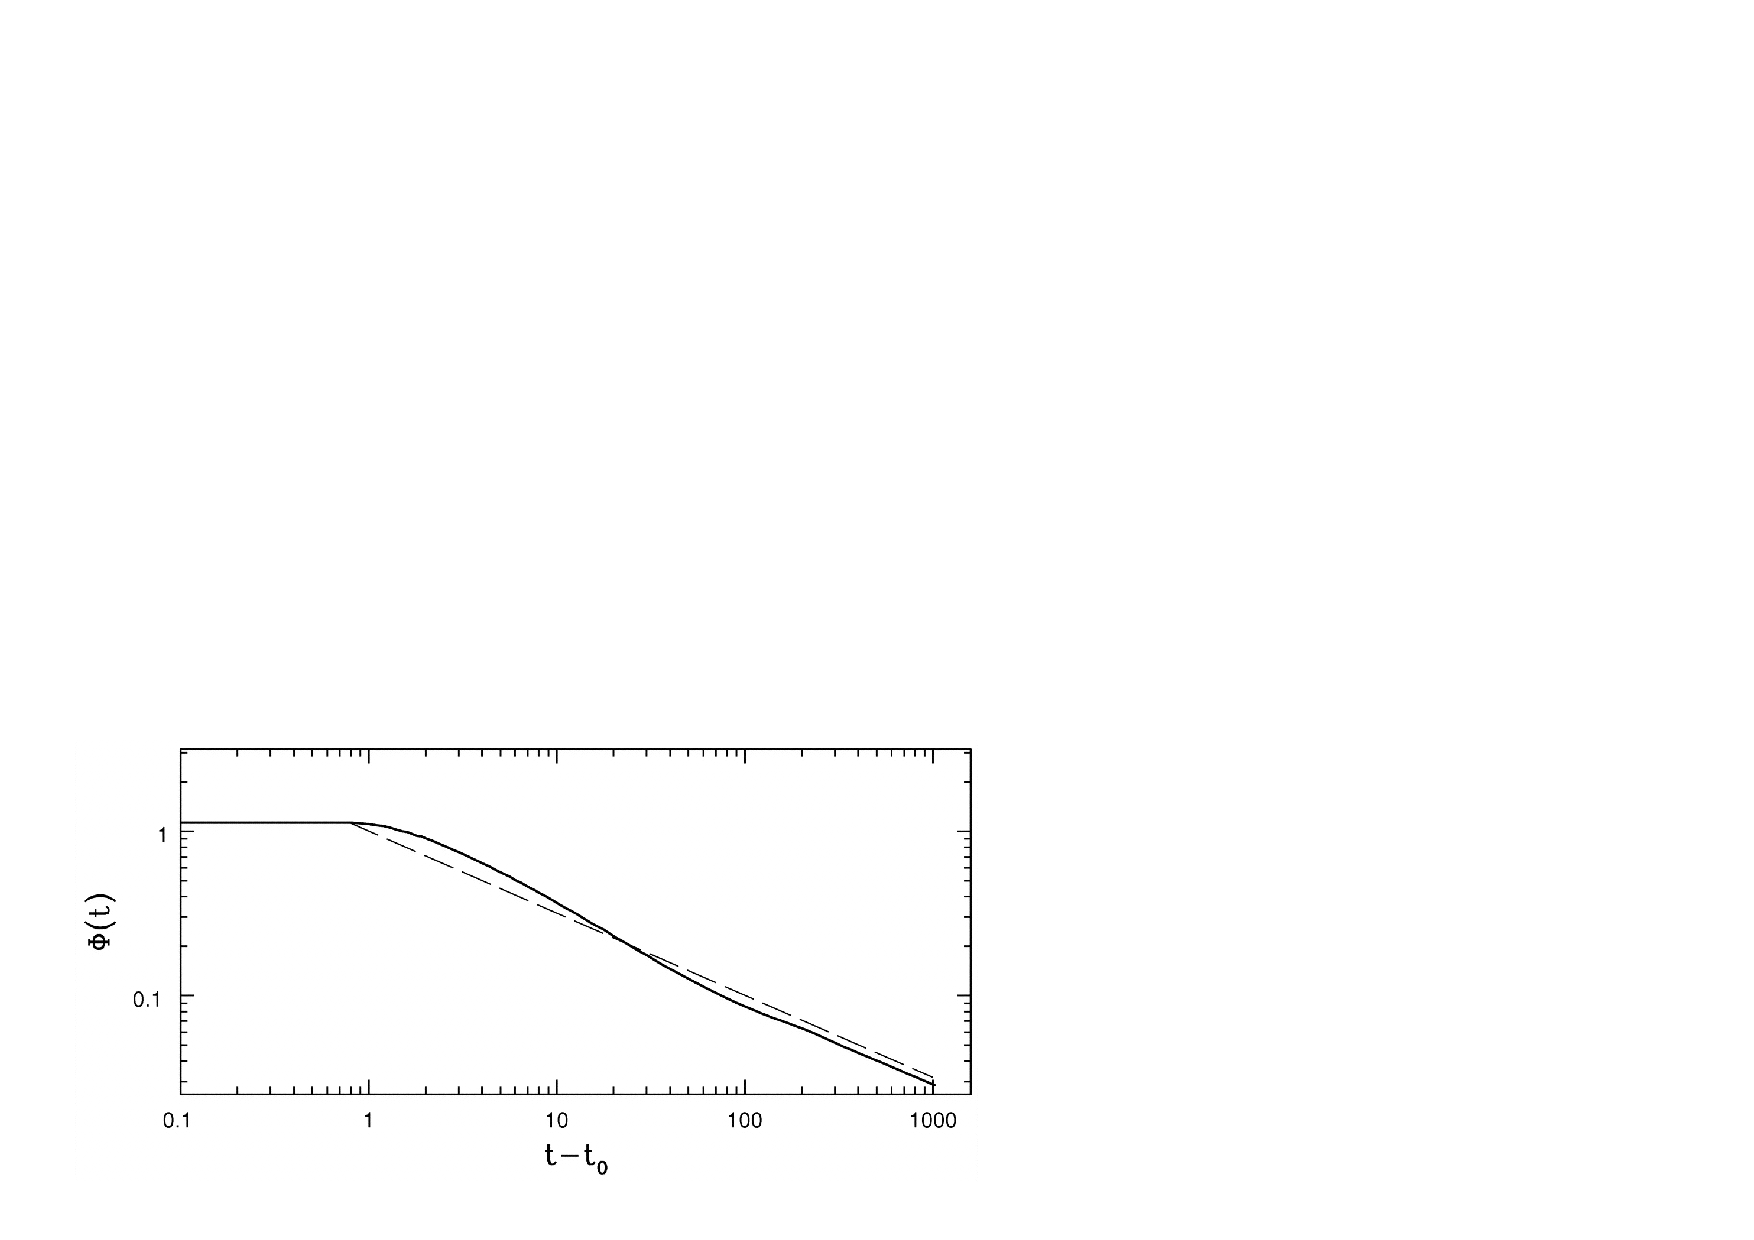
\includegraphics[width = 0.75\textwidth]{figures/AMF_burgers.pdf}
    \caption{Behaviour of the dimensionless AMF $\Phi(t)$ in the non-linear regime as a function of $t$ using $M_{\rm p} = M_1$ \citep[solid line;][]{rafikov2002a}.
    Before the shock is formed at approximately $t-t_0=1$ we see that $\Phi(t)$ is conserved, while decaying steadily after the shock is formed.
    The dashed line demonstrates that the AMF asymptotically scales as $\Phi(t) \propto t^{-1/2}$.
    }
    \label{fig:AMF}
\end{figure}

\subsection{Asymptotic Planet Mass Scaling}

While the AMF is no longer conserved in the dissipative wake evolution regime, Burger's equation does encode the perfect conservation of a quantity both before and after shock formation, which is the area under the curve $\chi$ \citep{landau1959,whitham1999}.
We will show that physically this corresponds to conservation of mass in the disk.
The area $\mathcal{A}$ under the curve at a ``time'' $t$ is given by
\begin{align}
    \mathcal{A} = \oint \chi \, d\eta = \frac{(\gamma + 1)g(r)r_{\rm p}}{2 \Sigma_0 l_{\rm p}} \int_0^{2\pi}  \left( \Sigma - \Sigma_0 \right) \, d\phi, 
\end{align}
where in the second equality we have used transformations \ref{eq:chi} and \ref{eq:eta}.
The second integral in the above must evaluate to zero by physical argument, since the perturbed density profile must have the same mass as the unperturbed profile $\int_0^{2 \pi} \Sigma \, d\phi = \int_0^{2 \pi} \Sigma_0 \, d\phi$.
Therefore the conservative properties of Burgers equation, that $\frac{d\mathcal{A}}{dt}=0$, ensures that the mass of each annulus in the disk is unchanged by the density perturbation.

Using this area conservation property \citet{bollati2021} derived an asymptotic solution for the N-wave profile of the planet wake in the limit of $t\rightarrow\infty$:
\begin{align}
    \chi(t, \eta) \sim \begin{dcases}
        \frac{\rm{sgn}\left(r - r_{\rm p}\right) \eta + \tilde{\eta}}{t - t_0} \quad &\rm{if} \, \eta \in \left[\eta_-, \eta_+ \right], \\
        0 \quad &\rm{else},
    \end{dcases}
\end{align}
where $\tilde{\eta} \simeq 2.96$ is the value of $\eta$ where the N-wave intersects the $\eta$-axis.
Additionally
\begin{align} 
    \eta_\pm &= - \rm{sgn}(r - r_{\rm p}) \tilde{\eta} \pm \sqrt{2 \mathcal{A} (t - t_0)}, \\
    \rm{where} \quad \mathcal{A} &= |C_0| \frac{\gamma + 1}{2^{3/4}} \frac{M_{\rm p}}{M_1},
\end{align}
and $C_0 \simeq -0.4$ is a numerically determined constant \citep{bollati2020}.

From this asymptotic solution one may determine a scaling relation for the planet mass in terms of only the distance the wake has propagated from the planet $t-t_0$ and the width of the wake $\eta_+ - \eta_-$, given by 
\begin{align}
    \frac{M_{\rm p}}{M_1} \propto \frac{\left( \eta_+ - \eta_- \right)^2}{t - t_0}. \label{eq:Mp_propto}
\end{align}
This scaling relation tells us the fundamental information that must be determined in order to constrain a planet mass from its wake observationally.
We see that we must know the reference mass $M_1$, as well as the transformations $t(r)$ and $\eta(r,\phi)$.
From this we may use equations \ref{eq:char_mass}, \ref{eq:t} and \ref{eq:eta} to produce a full list of basic quantities of the disk and planet system that must be determined:
\begin{enumerate}
    \item The rotation profile of the disk $\Omega(r)$ (although Keplerian is likely a good approximation),
    \item The unperturbed sound speed profile $c_0(r)$ OR the pressure scale height $H(r)$,
    \item The unperturbed surface density profile $\Sigma_0(r)$,
    \item The planet orbital radius $r_{\rm p}$,
    \item The planet azimuth $\phi_{\rm p}$.
\end{enumerate}
However, we note that from equation \ref{eq:phi_wake} that $c_0(r)$, $r_{\rm p}$ and $\phi_{\rm p}$ are all determined by the shape of the wake.
Therefore if we assume a disk to be Keplerian and fit the wake shape, all that remains is to determine $\Sigma_0$ and then $M_{\rm p}$ will be determined.
The most straightforward way to constrain this is through determining the size of the perturbation in $\chi$ which depends on $g(r)$ and so on $\Sigma_0$.
While at this stage it is not clear on how to extract the information from observations, this at least shows that the planet mass is determined entirely by the wake shape and amplitude.

Finally, while it is possible to calculate the scale factor for the proportionality relation \ref{eq:Mp_propto} from theory, the work of \citet{cimerman2021} suggests that this is better done through comparison with hydrodynamical simulations.

\section{Gap Opening} \label{sec:gap_opening}

For sufficiently large planets, the non-linear effects are such that the planet wake shocks immediately after formation and the solution can no longer be neatly separated into the linear generation and non-linear propagation regimes.
As already hinted at the condition under which this occurs in an inviscid disk is that the planet mass $M_{\rm p}$ exceeds the characteristic mass $M_1$ defined in equation \ref{eq:char_mass}.
For a Keplerian disk the minimum gap-opening mass is the thermal mass \citep{lin1993}, defined as \citep{goodman2001}
\begin{align}
    M_{\rm th} \equiv \frac{2}{3} \left( \frac{H_{\rm p}}{r_{\rm p}}  \right)^3 M_*. \label{eq:thermalmass}
\end{align}
Thus the wake solution approach presented in sections \ref{sec:linear_wake_excitation} and \ref{sec:nonlinear_evolution} is only \textit{strictly} valid for sub-thermal mass planets. It is not clear however, that the non-linear Burger's equation evolution is invalid for planets greater than the thermal mass. This non-linear prescription's strictest requirement is that the shock is sufficiently weak such that the perturbative approach is still valid.

Gap opening occurs because the dissipative shock fronts allow angular momentum from the material nearby the disk to be deposited elsewhere \citep{lin1979,goldreich1979,goldreich1980}.
The rough physical criterion for a gap to open depends on two conditions.
Firstly the Hill radius of the planet $r_{\rm H}$ \citep{hill1878} must fulfil $r_{\rm H} \gtrsim H$, known as the \textit{thermal condition}.
Secondly the transfer rate of angular momentum between the wake and disk must exceed the local transport rate from effective viscosity \citep{lin1993}.
The thermal condition is equivalent to $M_{\rm p} = M_{\rm th}$ while the second is irrelevant to discussions of inviscid disks.

\citet{kanagawa2015} found an analytic relation between planet mass $M_{\rm p}$, central star mass $M_*$, viscosity $\alpha$ \citep{shakura1973}, and gap depth $\Sigma_{\rm p} / \Sigma_0$ in the case of an axisymmetric and geometrically thin gas disk subject to viscous evolution
\begin{align}
    \frac{M_{\rm p}}{M_*} = 5 \times 10^{-4} \left( \frac{\Sigma_0}{\Sigma_{\rm p}} - 1 \right)^{\frac{1}{2}} \left( \frac{H_{\rm p}}{0.1}  \right)^{\frac{5}{2}} \left( \frac{\alpha}{10^{-3}} \right)^{\frac{1}{2}},
\end{align}
where the gap depth $\Sigma_{\rm p} / \Sigma_0$ is written in terms of the surface density in the gap $\Sigma_{\rm p}$, and the unperturbed surface density $\Sigma_0$.

The modern understanding of gap opening, considering both the effects of viscosity and non-linear planet wake evolution, states that the thermal condition is unnecessary.
Instead planets $\lesssim M_{\rm th}$ may be capable of opening a gap depending on the disk conditions \citep{rafikov2002}.
The opening criterion is given by \citep{kanagawa2015a}
\begin{align}
    M_{\rm p} \gtrsim 5 \left( \frac{H_{\rm p}}{r_{\rm p}} \right)^\frac{5}{2} \alpha^\frac{1}{2} M_*.
\end{align}
Hydrodynamical simulations have confirmed the ability of sub-thermal mass planets to open gaps \citep{duffell2013}.

Finally, gap-opening occurs not only in the gas component of disks, but also the dust component.
Dust gaps are actually far more pervasive observationally \citep[eg.][]{almapartnership2015,andrews2016,isella2016,andrews2018,huang2018b}, since the gas structure of a disk is less straightforward to probe \citep{miotello2022}.
Dust gaps can be created through the mechanisms already discussed, since the grains will migrate to the pressure maxima induced at the edges of the gas gap \citep{paardekooper2004}.
The large and weakly-coupled grains become trapped at these maxima.
Smaller grains couple to the gas strongly and so flow with it into the vicinity of the planet before being accreted \citep{paardekooper2006,fouchet2007}.
Additionally, gaps may be induced only in the dust the component.
Drag acts on dust grains interior and exterior to the planets orbit resulting in inward radial migration.
Exterior to the orbit the tidal torque induced by the planet resists the inward drift
\citep{dipierro2016}.
Dust grains are therefore cleared from near the planets orbit resulting in a dust gap.